
%% bare_conf.tex
%% V1.3
%% 2007/01/11
%% by Michael Shell
%% See:
%% http://www.michaelshell.org/
%% for current contact information.
%%
%% This is a skeleton file demonstrating the use of IEEEtran.cls
%% (requires IEEEtran.cls version 1.7 or later) with an IEEE conference paper.
%%
%% Support sites:
%% http://www.michaelshell.org/tex/ieeetran/
%% http://www.ctan.org/tex-archive/macros/latex/contrib/IEEEtran/
%% and
%% http://www.ieee.org/

%%*************************************************************************
%% Legal Notice:
%% This code is offered as-is without any warranty either expressed or
%% implied; without even the implied warranty of MERCHANTABILITY or
%% FITNESS FOR A PARTICULAR PURPOSE! 
%% User assumes all risk.
%% In no event shall IEEE or any contributor to this code be liable for
%% any damages or losses, including, but not limited to, incidental,
%% consequential, or any other damages, resulting from the use or misuse
%% of any information contained here.
%%
%% All comments are the opinions of their respective authors and are not
%% necessarily endorsed by the IEEE.
%%
%% This work is distributed under the LaTeX Project Public License (LPPL)
%% ( http://www.latex-project.org/ ) version 1.3, and may be freely used,
%% distributed and modified. A copy of the LPPL, version 1.3, is included
%% in the base LaTeX documentation of all distributions of LaTeX released
%% 2003/12/01 or later.
%% Retain all contribution notices and credits.
%% ** Modified files should be clearly indicated as such, including  **
%% ** renaming them and changing author support contact information. **
%%
%% File list of work: IEEEtran.cls, IEEEtran_HOWTO.pdf, bare_adv.tex,
%%                    bare_conf.tex, bare_jrnl.tex, bare_jrnl_compsoc.tex
%%*************************************************************************

% *** Authors should verify (and, if needed, correct) their LaTeX system  ***
% *** with the testflow diagnostic prior to trusting their LaTeX platform ***
% *** with production work. IEEE's font choices can trigger bugs that do  ***
% *** not appear when using other class files.                            ***
% The testflow support page is at:
% http://www.michaelshell.org/tex/testflow/



% Note that the a4paper option is mainly intended so that authors in
% countries using A4 can easily print to A4 and see how their papers will
% look in print - the typesetting of the document will not typically be
% affected with changes in paper size (but the bottom and side margins will).
% Use the testflow package mentioned above to verify correct handling of
% both paper sizes by the user's LaTeX system.
%
% Also note that the "draftcls" or "draftclsnofoot", not "draft", option
% should be used if it is desired that the figures are to be displayed in
% draft mode.
%
\documentclass[10pt, conference, compsocconf]{IEEEtran}
% Add the compsocconf option for Computer Society conferences.
%
% If IEEEtran.cls has not been installed into the LaTeX system files,
% manually specify the path to it like:
% \documentclass[conference]{../sty/IEEEtran}





% Some very useful LaTeX packages include:
% (uncomment the ones you want to load)


% *** MISC UTILITY PACKAGES ***
%
%\usepackage{ifpdf}
% Heiko Oberdiek's ifpdf.sty is very useful if you need conditional
% compilation based on whether the output is pdf or dvi.
% usage:
% \ifpdf
%   % pdf code
% \else
%   % dvi code
% \fi
% The latest version of ifpdf.sty can be obtained from:
% http://www.ctan.org/tex-archive/macros/latex/contrib/oberdiek/
% Also, note that IEEEtran.cls V1.7 and later provides a builtin
% \ifCLASSINFOpdf conditional that works the same way.
% When switching from latex to pdflatex and vice-versa, the compiler may
% have to be run twice to clear warning/error messages.






% *** CITATION PACKAGES ***
%
%\usepackage{cite}
% cite.sty was written by Donald Arseneau
% V1.6 and later of IEEEtran pre-defines the format of the cite.sty package
% \cite{} output to follow that of IEEE. Loading the cite package will
% result in citation numbers being automatically sorted and properly
% "compressed/ranged". e.g., [1], [9], [2], [7], [5], [6] without using
% cite.sty will become [1], [2], [5]--[7], [9] using cite.sty. cite.sty's
% \cite will automatically add leading space, if needed. Use cite.sty's
% noadjust option (cite.sty V3.8 and later) if you want to turn this off.
% cite.sty is already installed on most LaTeX systems. Be sure and use
% version 4.0 (2003-05-27) and later if using hyperref.sty. cite.sty does
% not currently provide for hyperlinked citations.
% The latest version can be obtained at:
% http://www.ctan.org/tex-archive/macros/latex/contrib/cite/
% The documentation is contained in the cite.sty file itself.






% *** GRAPHICS RELATED PACKAGES ***
%
\ifCLASSINFOpdf
  % \usepackage[pdftex]{graphicx}
  % declare the path(s) where your graphic files are
  % \graphicspath{{../pdf/}{../jpeg/}}
  % and their extensions so you won't have to specify these with
  % every instance of \includegraphics
  % \DeclareGraphicsExtensions{.pdf,.jpeg,.png}
\else
  % or other class option (dvipsone, dvipdf, if not using dvips). graphicx
  % will default to the driver specified in the system graphics.cfg if no
  % driver is specified.
  % \usepackage[dvips]{graphicx}
  % declare the path(s) where your graphic files are
  % \graphicspath{{../eps/}}
  % and their extensions so you won't have to specify these with
  % every instance of \includegraphics
  % \DeclareGraphicsExtensions{.eps}
\fi
% graphicx was written by David Carlisle and Sebastian Rahtz. It is
% required if you want graphics, photos, etc. graphicx.sty is already
% installed on most LaTeX systems. The latest version and documentation can
% be obtained at: 
% http://www.ctan.org/tex-archive/macros/latex/required/graphics/
% Another good source of documentation is "Using Imported Graphics in
% LaTeX2e" by Keith Reckdahl which can be found as epslatex.ps or
% epslatex.pdf at: http://www.ctan.org/tex-archive/info/
%
% latex, and pdflatex in dvi mode, support graphics in encapsulated
% postscript (.eps) format. pdflatex in pdf mode supports graphics
% in .pdf, .jpeg, .png and .mps (metapost) formats. Users should ensure
% that all non-photo figures use a vector format (.eps, .pdf, .mps) and
% not a bitmapped formats (.jpeg, .png). IEEE frowns on bitmapped formats
% which can result in "jaggedy"/blurry rendering of lines and letters as
% well as large increases in file sizes.
%
% You can find documentation about the pdfTeX application at:
% http://www.tug.org/applications/pdftex





% *** MATH PACKAGES ***
%
%\usepackage[cmex10]{amsmath}
% A popular package from the American Mathematical Society that provides
% many useful and powerful commands for dealing with mathematics. If using
% it, be sure to load this package with the cmex10 option to ensure that
% only type 1 fonts will utilized at all point sizes. Without this option,
% it is possible that some math symbols, particularly those within
% footnotes, will be rendered in bitmap form which will result in a
% document that can not be IEEE Xplore compliant!
%
% Also, note that the amsmath package sets \interdisplaylinepenalty to 10000
% thus preventing page breaks from occurring within multiline equations. Use:
%\interdisplaylinepenalty=2500
% after loading amsmath to restore such page breaks as IEEEtran.cls normally
% does. amsmath.sty is already installed on most LaTeX systems. The latest
% version and documentation can be obtained at:
% http://www.ctan.org/tex-archive/macros/latex/required/amslatex/math/





% *** SPECIALIZED LIST PACKAGES ***
%
%\usepackage{algorithmic}
% algorithmic.sty was written by Peter Williams and Rogerio Brito.
% This package provides an algorithmic environment fo describing algorithms.
% You can use the algorithmic environment in-text or within a figure
% environment to provide for a floating algorithm. Do NOT use the algorithm
% floating environment provided by algorithm.sty (by the same authors) or
% algorithm2e.sty (by Christophe Fiorio) as IEEE does not use dedicated
% algorithm float types and packages that provide these will not provide
% correct IEEE style captions. The latest version and documentation of
% algorithmic.sty can be obtained at:
% http://www.ctan.org/tex-archive/macros/latex/contrib/algorithms/
% There is also a support site at:
% http://algorithms.berlios.de/index.html
% Also of interest may be the (relatively newer and more customizable)
% algorithmicx.sty package by Szasz Janos:
% http://www.ctan.org/tex-archive/macros/latex/contrib/algorithmicx/




% *** ALIGNMENT PACKAGES ***
%
%\usepackage{array}
% Frank Mittelbach's and David Carlisle's array.sty patches and improves
% the standard LaTeX2e array and tabular environments to provide better
% appearance and additional user controls. As the default LaTeX2e table
% generation code is lacking to the point of almost being broken with
% respect to the quality of the end results, all users are strongly
% advised to use an enhanced (at the very least that provided by array.sty)
% set of table tools. array.sty is already installed on most systems. The
% latest version and documentation can be obtained at:
% http://www.ctan.org/tex-archive/macros/latex/required/tools/


%\usepackage{mdwmath}
%\usepackage{mdwtab}
% Also highly recommended is Mark Wooding's extremely powerful MDW tools,
% especially mdwmath.sty and mdwtab.sty which are used to format equations
% and tables, respectively. The MDWtools set is already installed on most
% LaTeX systems. The lastest version and documentation is available at:
% http://www.ctan.org/tex-archive/macros/latex/contrib/mdwtools/


% IEEEtran contains the IEEEeqnarray family of commands that can be used to
% generate multiline equations as well as matrices, tables, etc., of high
% quality.


%\usepackage{eqparbox}
% Also of notable interest is Scott Pakin's eqparbox package for creating
% (automatically sized) equal width boxes - aka "natural width parboxes".
% Available at:
% http://www.ctan.org/tex-archive/macros/latex/contrib/eqparbox/





% *** SUBFIGURE PACKAGES ***
%\usepackage[tight,footnotesize]{subfigure}
% subfigure.sty was written by Steven Douglas Cochran. This package makes it
% easy to put subfigures in your figures. e.g., "Figure 1a and 1b". For IEEE
% work, it is a good idea to load it with the tight package option to reduce
% the amount of white space around the subfigures. subfigure.sty is already
% installed on most LaTeX systems. The latest version and documentation can
% be obtained at:
% http://www.ctan.org/tex-archive/obsolete/macros/latex/contrib/subfigure/
% subfigure.sty has been superceeded by subfig.sty.



%\usepackage[caption=false]{caption}
%\usepackage[font=footnotesize]{subfig}
% subfig.sty, also written by Steven Douglas Cochran, is the modern
% replacement for subfigure.sty. However, subfig.sty requires and
% automatically loads Axel Sommerfeldt's caption.sty which will override
% IEEEtran.cls handling of captions and this will result in nonIEEE style
% figure/table captions. To prevent this problem, be sure and preload
% caption.sty with its "caption=false" package option. This is will preserve
% IEEEtran.cls handing of captions. Version 1.3 (2005/06/28) and later 
% (recommended due to many improvements over 1.2) of subfig.sty supports
% the caption=false option directly:
%\usepackage[caption=false,font=footnotesize]{subfig}
%
% The latest version and documentation can be obtained at:
% http://www.ctan.org/tex-archive/macros/latex/contrib/subfig/
% The latest version and documentation of caption.sty can be obtained at:
% http://www.ctan.org/tex-archive/macros/latex/contrib/caption/




% *** FLOAT PACKAGES ***
%
%\usepackage{fixltx2e}
% fixltx2e, the successor to the earlier fix2col.sty, was written by
% Frank Mittelbach and David Carlisle. This package corrects a few problems
% in the LaTeX2e kernel, the most notable of which is that in current
% LaTeX2e releases, the ordering of single and double column floats is not
% guaranteed to be preserved. Thus, an unpatched LaTeX2e can allow a
% single column figure to be placed prior to an earlier double column
% figure. The latest version and documentation can be found at:
% http://www.ctan.org/tex-archive/macros/latex/base/



%\usepackage{stfloats}
% stfloats.sty was written by Sigitas Tolusis. This package gives LaTeX2e
% the ability to do double column floats at the bottom of the page as well
% as the top. (e.g., "\begin{figure*}[!b]" is not normally possible in
% LaTeX2e). It also provides a command:
%\fnbelowfloat
% to enable the placement of footnotes below bottom floats (the standard
% LaTeX2e kernel puts them above bottom floats). This is an invasive package
% which rewrites many portions of the LaTeX2e float routines. It may not work
% with other packages that modify the LaTeX2e float routines. The latest
% version and documentation can be obtained at:
% http://www.ctan.org/tex-archive/macros/latex/contrib/sttools/
% Documentation is contained in the stfloats.sty comments as well as in the
% presfull.pdf file. Do not use the stfloats baselinefloat ability as IEEE
% does not allow \baselineskip to stretch. Authors submitting work to the
% IEEE should note that IEEE rarely uses double column equations and
% that authors should try to avoid such use. Do not be tempted to use the
% cuted.sty or midfloat.sty packages (also by Sigitas Tolusis) as IEEE does
% not format its papers in such ways.





% *** PDF, URL AND HYPERLINK PACKAGES ***
%
%\usepackage{url}
% url.sty was written by Donald Arseneau. It provides better support for
% handling and breaking URLs. url.sty is already installed on most LaTeX
% systems. The latest version can be obtained at:
% http://www.ctan.org/tex-archive/macros/latex/contrib/misc/
% Read the url.sty source comments for usage information. Basically,
% \url{my_url_here}.





% *** Do not adjust lengths that control margins, column widths, etc. ***
% *** Do not use packages that alter fonts (such as pslatex).         ***
% There should be no need to do such things with IEEEtran.cls V1.6 and later.
% (Unless specifically asked to do so by the journal or conference you plan
% to submit to, of course. )

\usepackage{times}
\usepackage{graphicx}
\usepackage{epsf}
\usepackage{verbatim}
\usepackage{psfig}
\usepackage{cite}
\usepackage{url}
\usepackage{color}
\usepackage{alltt}

\usepackage{longtable,lscape}
\usepackage{slashbox,multirow}
\usepackage{colortbl}
\usepackage{mathrsfs}

\newcommand{\Add}{\CodeIn{add}}
\newcommand{\AVTree}{\CodeIn{AVTree}}
\newcommand{\Assignment}[3]{$\langle$ \Object{#1}, \Object{#2}, \Object{#3} $\rangle$}
\newcommand{\BinaryTreeRemove}{\CodeIn{BinaryTree\_remove}}
\newcommand{\BinaryTree}{\CodeIn{BinaryTree}}
\newcommand{\Caption}{\caption}
\newcommand{\Char}[1]{`#1'}
\newcommand{\CheckRep}{\CodeIn{checkRep}}
\newcommand{\ClassC}{\CodeIn{C}}
\newcommand{\CodeIn}[1]{{\small\texttt{#1}}}
\newcommand{\CodeOutSize}{\scriptsize}
\newcommand{\Comment}[1]{}
\newcommand{\Ensures}{\CodeIn{ensures}}
\newcommand{\ExtractMax}{\CodeIn{extractMax}}
\newcommand{\FAL}{field-ordering}
\newcommand{\FALs}{field-orderings}
\newcommand{\Fact}{observation}
\newcommand{\Get}{\CodeIn{get}}
\newcommand{\HashSet}{\CodeIn{HashSet}}
\newcommand{\HeapArray}{\CodeIn{HeapArray}}
\newcommand{\Intro}[1]{\emph{#1}}
\newcommand{\Invariant}{\CodeIn{invariant}}
\newcommand{\JUC}{\CodeIn{java.\-util.\-Collections}}
\newcommand{\JUS}{\CodeIn{java.\-util.\-Set}}
\newcommand{\JUTM}{\CodeIn{java.\-util.\-TreeMap}}
\newcommand{\JUTS}{\CodeIn{java.\-util.\-TreeSet}}
\newcommand{\JUV}{\CodeIn{java.\-util.\-Vector}}
\newcommand{\JMLPlusJUnit}{JML+JUnit}
\newcommand{\Korat}{Korat}
\newcommand{\Left}{\CodeIn{left}}
\newcommand{\Lookup}{\CodeIn{lookup}}
\newcommand{\MethM}{\CodeIn{m}}
\newcommand{\Node}[1]{\CodeIn{N}$_#1$}
\newcommand{\Null}{\CodeIn{null}}
\newcommand{\Object}[1]{\CodeIn{o}\ensuremath{_#1}}
\newcommand{\PostM}{\MethM$_{post}$}
\newcommand{\PreM}{\MethM$_{pre}$}
\newcommand{\Put}{\CodeIn{put}}
\newcommand{\Remove}{\CodeIn{remove}}
\newcommand{\RepOk}{\CodeIn{repOk}}
\newcommand{\Requires}{\CodeIn{requires}}
\newcommand{\Reverse}{\CodeIn{reverse}}
\newcommand{\Right}{\CodeIn{right}}
\newcommand{\Root}{\CodeIn{root}}
\newcommand{\Set}{\CodeIn{set}}
\newcommand{\State}[1]{2^{#1}}
\newcommand{\TestEra}{TestEra}
\newcommand{\TreeMap}{\CodeIn{TreeMap}}

\newenvironment{CodeOut}{\begin{scriptsize}}{\end{scriptsize}}
\newenvironment{SmallOut}{\begin{small}}{\end{small}}

\newcommand{\pairwiseEquals}{PairwiseEquals}
\newcommand{\monitorEquals}{MonitorEquals}
%\newcommand{\monitorWField}{WholeStateW}
\newcommand{\traverseField}{WholeState}
\newcommand{\monitorSMSeq}{ModifyingSeq}
\newcommand{\monitorSeq}{WholeSeq}

\newcommand{\IntStack}{\CodeIn{IntStack}}
\newcommand{\UBStack}{\CodeIn{UBStack}}
\newcommand{\BSet}{\CodeIn{BSet}}
\newcommand{\BBag}{\CodeIn{BBag}}
\newcommand{\ShoppingCart}{\CodeIn{ShoppingCart}}
\newcommand{\BankAccount}{\CodeIn{BankAccount}}
\newcommand{\BinarySearchTree}{\CodeIn{BinarySearchTree}}
\newcommand{\LinkedList}{\CodeIn{LinkedList}}

\newcommand{\Book}{\CodeIn{Book}}
\newcommand{\Library}{\CodeIn{Library}}

\newcommand{\Jtest}{Jtest}
\newcommand{\JCrasher}{JCrasher}
\newcommand{\Daikon}{Daikon}
\newcommand{\JUnit}{JUnit}

\newcommand{\trie}{trie}

\newcommand{\Perl}{Perl}


\newcommand{\SubjectCount}{11}
\newcommand{\DSSubjectCount}{two}

\newcommand{\Equals}{\CodeIn{equals}}
\newcommand{\Pairwise}{PairwiseEquals}
\newcommand{\Subgraph}{MonitorEquals}
\newcommand{\Concrete}{WholeState}
\newcommand{\ModSeq}{ModifyingSeq}
\newcommand{\Seq}{WholeSeq}
\newcommand{\Aeq}{equality}

\newcommand{\Meaning}[1]{\ensuremath{[\![}#1\ensuremath{]\!]}}
\newcommand{\Pair}[2]{\ensuremath{\langle #1, #2 \rangle}}
\newcommand{\Triple}[3]{\ensuremath{\langle #1, #2, #3 \rangle}}
\newcommand{\SetSuch}[2]{\ensuremath{\{ #1 | #2 \}}}

\newcommand{\Equiv}[2]{\ensuremath{#1 \EquivSTRel{} #2}}
\newcommand{\EquivME}{\Equiv}
\newcommand{\EquivST}{\Equiv}
\newcommand{\EquivSTRel}{\ensuremath{\cong}}
\newcommand{\Redundant}[2]{\ensuremath{#1 \lhd #2}}
\newcommand{\VB}{\ensuremath{\mid}}
\newcommand{\MES}{method-entry state}

\newcommand{\Small}[1]{{\small{#1}}}

\newcommand{\CenterCell}[1]{\multicolumn{1}{c|}{#1}}


\begin{document}
%
% paper title
% can use linebreaks \\ within to get better formatting as desired
\title{Alattin: Mining Alternative Patterns for Detecting Neglected Conditions}


% author names and affiliations
% use a multiple column layout for up to two different
% affiliations

\author{\IEEEauthorblockN{Suresh Thummalapenta}
\IEEEauthorblockA{Department of Computer Science\\
North Carolina State University\\
Raleigh, USA\\
sthumma@ncsu.edu}
\and
\IEEEauthorblockN{Tao Xie}
\IEEEauthorblockA{Department of Computer Science\\
North Carolina State University\\
Raleigh, USA\\
xie@csc.ncsu.edu}
}

% conference papers do not typically use \thanks and this command
% is locked out in conference mode. If really needed, such as for
% the acknowledgment of grants, issue a \IEEEoverridecommandlockouts
% after \documentclass

% for over three affiliations, or if they all won't fit within the width
% of the page, use this alternative format:
% 
%\author{\IEEEauthorblockN{Michael Shell\IEEEauthorrefmark{1},
%Homer Simpson\IEEEauthorrefmark{2},
%James Kirk\IEEEauthorrefmark{3}, 
%Montgomery Scott\IEEEauthorrefmark{3} and
%Eldon Tyrell\IEEEauthorrefmark{4}}
%\IEEEauthorblockA{\IEEEauthorrefmark{1}School of Electrical and Computer Engineering\\
%Georgia Institute of Technology,
%Atlanta, Georgia 30332--0250\\ Email: see http://www.michaelshell.org/contact.html}
%\IEEEauthorblockA{\IEEEauthorrefmark{2}Twentieth Century Fox, Springfield, USA\\
%Email: homer@thesimpsons.com}
%\IEEEauthorblockA{\IEEEauthorrefmark{3}Starfleet Academy, San Francisco, California 96678-2391\\
%Telephone: (800) 555--1212, Fax: (888) 555--1212}
%\IEEEauthorblockA{\IEEEauthorrefmark{4}Tyrell Inc., 123 Replicant Street, Los Angeles, California 90210--4321}}




% use for special paper notices
%\IEEEspecialpapernotice{(Invited Paper)}




% make the title area
\maketitle


\begin{abstract}

Software developers often face
challenges in reusing open source frameworks due to several factors
such as the framework complexity and lack of proper
documentation. In this paper, we propose a code-search-engine-based
approach that detects \Intro{hotspots} in a given framework
by mining code examples gathered from open source repositories available on the web; 
these hotspots are API classes and methods that are frequently reused. 
Hotspots can serve as starting points for developers
in understanding and reusing the given framework. 
Our approach also detects \Intro{coldspots}, which are API classes and methods that are rarely used.
Coldspots serve as caveats for developers as there can 
be difficulties in finding relevant code examples and are generally less exercised
compared to hotspots. We developed a tool, called SpotWeb, for
frameworks or libraries written in Java and used our tool
to detect hotspots and coldspots of eight widely used open source
frameworks. We show the utility of our detected hotspots 
by comparing these hotspots with the API classes reused by a real application
and compare our results with the results of a previous related approach.
\end{abstract}


\begin{IEEEkeywords}
code search; frequent itemset mining; alternative patterns;
\end{IEEEkeywords}

\section{Introduction}
\label{sec:intro}
\vspace*{-3ex}
Programming languages such as Java and C++ provide exception-handling 
constructs such as \CodeIn{try-catch} to handle exception conditions that arise
during program execution. Under these exception conditions, programs follow paths
different from normal execution paths; these additional paths are referred to as 
\emph{exception} paths. Applications developed based on these programming
languages are expected to handle these exception conditions and take necessary recovery
actions. For example, when an application reuses resources such as files or database connections,
the application should release the resources after the usage in all paths
including \Intro{exception} paths. Failing to release the resources can not only cause performance degradation, 
but can also lead to critical issues. For example, if a database lock acquired by a
process is not released, any other process trying to acquire the same lock
hangs till the database releases the lock after timeout.
A case study~\cite{Weimer04} conducted on a real application 
demonstrates the necessity of releasing resources in exception paths 
for improving reliability and performance. 
The case study found that there was a surprising
improvement of 17\% in performance of the application after 
correctly releasing resources in the presence of exceptions.

\Comment{In general, software verification concentrates on verifying behaviors of the application 
during normal execution paths rather than exception paths. Therefore, the exception 
cases remain undetected during traditional software verification.}

Software verification can be challenging for exception cases as verification
techniques require specifications that describe expected behaviors when exceptions occur.
These specifications are often not available in practice~\cite{document:leth}.
To address this issue, association rules of the form ``$FC_a$ $\Rightarrow$ $FC_e$''
are mined as specifications~\cite{WeimerN05}, where both $FC_a$ and $FC_e$ are function calls that share
the same receiver object. These specifications are used to 
verify whether the function call $FC_a$ is followed by the function call $FC_e$ in all 
exception paths. However, simple association rules of this form are often not sufficient
to characterize common exception-handling rules. The rationale is that
there are various scenarios where $FC_a$ is not necessarily followed by $FC_e$ 
when exceptions are raised by $FC_a$, although both function calls 
share the same receiver object. 

\begin{figure*}[t]
\centering
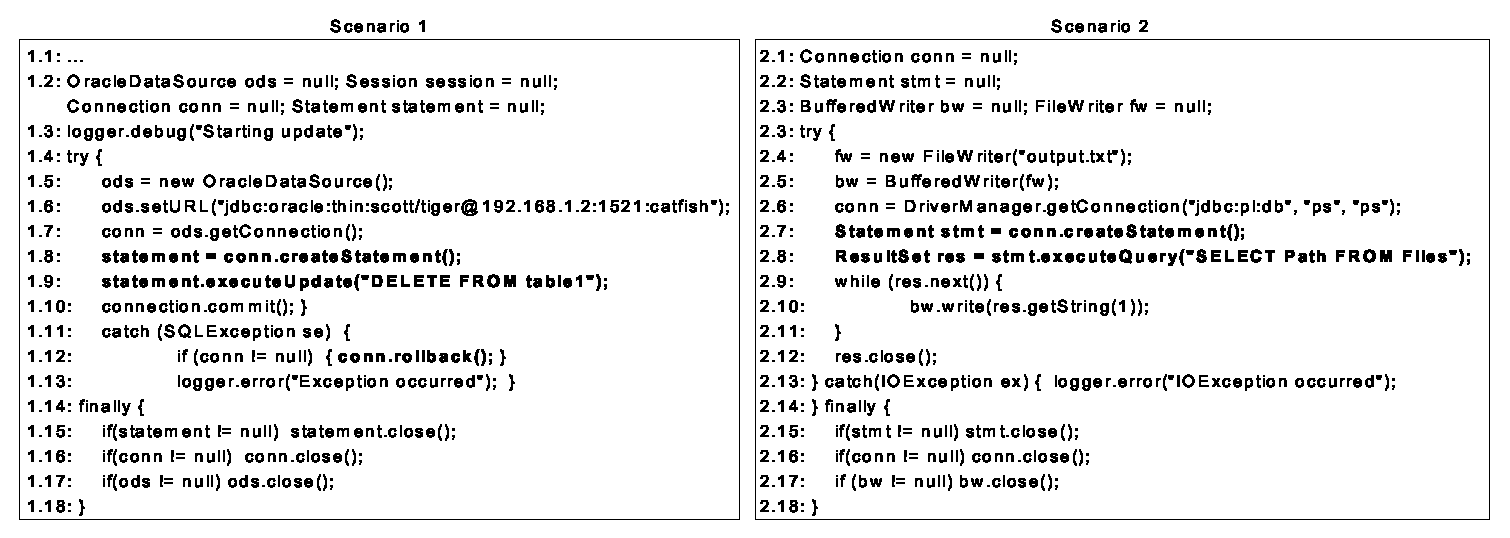
\includegraphics[scale=0.70,clip]{figs/three-code-examples1.eps}\vspace*{-3ex}
\centering \caption {\label{fig:threescenarios} Two example scenarios from real applications.}\vspace*{-4ex}
\end{figure*}

We next present an example using Scenarios 1 and 2 (extracted 
from real applications) shown in Figure~\ref{fig:threescenarios}. 
Scenario 1 attempts to modify contents of a database through the function call
\CodeIn{Statement.executeUpdate} (Line 1.9), whereas Scenario 2 attempts to read contents
of a database through the function call \CodeIn{Statement.executeQuery} (Line 2.8).
Consider a simple specification in the form of an association
rule ``\CodeIn{Connection creation} $\Rightarrow$
\CodeIn{Connection rollback}''. This rule describes that a \CodeIn{rollback} function call should
appear in exception paths whenever an object of \CodeIn{Connection} is created. 
Although a \CodeIn{Connection} object is created in both
scenarios, this rule applies only to Scenario 1 and does not apply to Scenario 2.
The primary reason is that the \CodeIn{rollback} function call should be invoked \emph{only} when 
there are any changes made to the database. This example shows that
simple association rules of the form ``$FC_a$ $\Rightarrow$ $FC_e$''
are often insufficient to characterize exception-handling rules.

The insufficiency of simple association rules calls for 
more general association rules, hereby referred to as \Intro{sequence association rules},
of the form ``($FC_c^1$...$FC_c^n$) $\wedge$ $FC_a$ $\Rightarrow$ ($FC_e^1$...$FC_e^m$)''.
This sequence association rule describes that function call $FC_a$ should be followed 
by function-call sequence $FC_e^1$...$FC_e^m$ in exception paths only 
when preceded by function-call sequence $FC_c^1$...$FC_c^n$. Using this sequence association rule,
the preceding example can be expressed as ``($FC_c^1$$FC_c^2$) $\wedge$ 
$FC_a$ $\Rightarrow$ ($FC_e^1$)'', where

$FC_c^1$ : \CodeIn{OracleDataSource.getConnection}\\
\hspace*{0.15in}$FC_c^2$ : \CodeIn{Connection.createStatement}\\
\hspace*{0.15in}$FC_a$ : \CodeIn{Statement.executeUpdate}\\
\hspace*{0.15in}$FC_e^1$ : \CodeIn{Connection.rollback}\\
\vspace*{-2ex}

This sequence association rule applies to Scenario 1 and
does not apply to Scenario 2 due to the presence of $FC_a$: \CodeIn{Statement.executeUpdate}.
The key aspects to be noted in this rule are: (1) \CodeIn{Statement.executeUpdate}
is the primary reason to have \CodeIn{Connection.rollback} in an exception path and
(2) the receiver object of \CodeIn{Statement.executeUpdate} is dependent on the 
receiver object of \CodeIn{Connection.rollback} through the function-call sequence
defined by $FC_c^1$$FC_c^2$.

Our sequence association rules are a super set of simple association rules.
For example, sequence association rules are the same as simple association
rules when the sequence $FC_c^1$...$FC_c^n$ is empty. 
To the best of our knowledge, existing association rule mining techniques~\cite{agarwal:association}
cannot be directly applied to mine these sequence association rules. 
Therefore, to bridge the gap, we develop a new mining algorithm by adapting the
frequent closed subsequence mining technique~\cite{wang:bide}. 

We further develop a novel approach, called CAR-Miner, that incorporates
our new mining algorithm for the problem of detecting exception-handling rules in
the form of sequence association rules by analyzing source code. Apart from mining sequence
association rules, CAR-Miner addresses another challenge that is often faced 
by existing approaches~\cite{Zhenmin2005PRMiner, chang07:finding, WeimerN05}, 
which mine rules from a limited data scope, 
i.e., from only a few example applications. Therefore, these approaches may not 
be able to mine rules that do not have enough
supporting samples in those example applications, and hence 
the related defects remain undetected by these approaches. To address
this challenge, CAR-Miner expands the data scope by leveraging a code search engine (CSE)
for gathering relevant code samples from existing open source projects available
on the web. From these relevant code samples, CAR-Miner mines exception-handling rules. 
We show the usefulness of mined exception-handling rules
by applying these rules on five applications to detect violations.
CAR-Miner tries to address problems related to the quality of code samples 
gathered from a CSE by capturing the most frequent patterns through mining.

\Comment{In particular, CAR-Miner accepts an input application and tries to detect
exception-handling defects in that application. Initially, CAR-Miner gathers function calls, referred as
$FC_a$, used by  the input application. CAR-Miner interacts with a code search engine (CSE) such as Google code search~\cite{GCSE} to gather related code examples that are already reusing $FC_a$. 
CAR-Miner constructs an Exception Flow Graph (EFG) for each code example gathered from 
the CSE. EFG is an extended form of control flow graph that captures flow of control in both
normal and exception conditions. While constructing EFG, we add only those exception
paths that can occur potentially during program execution. To capture such
exception paths, we use a sound static analysis that provides a set
of exceptions thrown by each $FC_a$ during program execution. 
CAR-Miner collects traces, which are
in the form of a sequence of function calls, from EFG post-processes these 
traces to filter unrelated function calls of $FC_a$.
CAR-Miner mines these traces to capture sequence association rules. 
Finally, CAR-Miner applies mined exception-handling rules to detect violations in the input application.
As CAR-Miner leverages a code search engine for gathering related code examples,
CAR-Miner has an added advantage of being able to mine rules, which do not have enough
supporting samples in the input application. CAR-Miner tries to address the 
problems related to the quality of the code examples 
gathered from a CSE by capturing the most frequent rule candidates through mining.}

This paper makes the following main contributions:\vspace*{-1ex}
\begin{Itemize}
\item A general mining algorithm to mine sequence association rules of the form 
``($FC_c^1$...$FC_c^n$) $\wedge$ $FC_a$ $\Rightarrow$ ($FC_e^1$...$FC_e^m$)''.
Our new mining algorithm takes a step forward in the direction 
of developing new mining algorithms to address
unique requirements in mining software engineering data, beyond being limited
by existing off-the-shelf mining algorithms.\vspace*{-2ex}
\item An approach that incorporates the general mining algorithm to mine exception-handling
rules that describe expected behavior when exceptions occur during
program execution. \vspace*{-2ex}
\item A technique for constructing a precise Exception-Flow Graph (EFG), which is an extended form of 
a Control-Flow Graph (CFG), that includes only those exception paths that can potentially occur 
during program execution.\vspace*{-2ex}
\item An implementation for expanding the data scope to open source projects that help
detect new related exception-handling rules that do not have enough supporting samples in an application under analysis.
These rules can help detect new defects in the application under analysis.\vspace*{-2ex}
\item Two evaluations to show
the effectiveness of our approach. (1) CAR-Miner detects $294$ real 
exception-handling rules in five different applications including $285$ KLOC. 
(2) The top $50$ exception-handling
rules (top $10$ real rules of each application)
are used to detect a total of $160$ real defects in these five
applications, where $87$ defects are new, not being detected by a 
previous related approach~\cite{WeimerN05}. \Comment{The initial response from 
developers of HsqlDB~\footnote{\url{http://hsqldb.sourceforge.net/}} is
encouraging. The developers responded on the first ten defects that we reported, 
where seven defects are \emph{accepted} and only three defects are rejected.}
\end{Itemize}

The rest of the paper is organized as follows. 
%Section~\ref{sec:example} presents example scenarios.
Section~\ref{sec:condrules} presents a formal definition of sequence
association rules and describes our new mining algorithm.
Section~\ref{sec:approach} describes key aspects of the CAR-Miner approach.
Section~\ref{sec:eval} presents evaluation results.
%Section~\ref{sec:discussion} presents limitations and future work.
Section~\ref{sec:threats} discusses threats to validity.
Section~\ref{sec:related} presents related work.
Finally, Section~\ref{sec:conclusion} concludes.



\section{ImMiner Algorithm}
\label{sec:imminer}

We next present an example to explain the major concepts of our ImMiner algorithm and then present a formal definition of the problem addressed by our mining algorithm.

%-----------------------------------------------------------------------
\subsection{Example}

\begin{figure}[t]
\centering
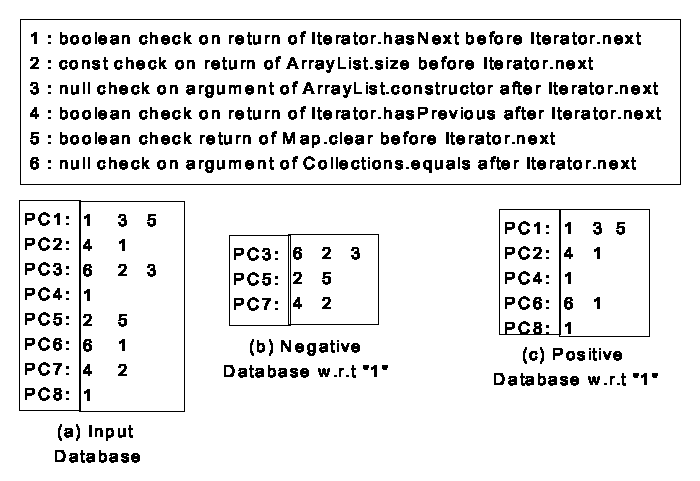
\includegraphics[scale=0.75,clip]{figs/miningex1.eps}\vspace*{-1ex}
\caption{Example for the \CodeIn{Iterator.next} API method used to illustrate our mining algorithm} \label{fig:miningex}
\vspace*{-1ex}
\end{figure}

Figure~\ref{fig:miningex}a shows an input database for applying our mining algorithm, where each row includes the surrounding condition checks (i.e., condition checks before or after an API call) of the same API method from a code example. We refer to each row in the input database as a pattern candidate (PC). For example, PC1 describes that three condition checks are done before and after invoking \CodeIn{Iterator.next}. Given such input database, ImMiner uses two steps for mining alternative patterns of the form ``$P_1$ \textbf{or} $\hat{P_2}$'', where $P_1$ represents ``\CodeIn{boolean check} on the return of \CodeIn{Iterator.hasNext} before \CodeIn{Iterator.next}'' and $P_2$ represents ``\CodeIn{const check} on the return of \CodeIn{ArrayList.size} before \CodeIn{Iterator.next}''.

In Step 1, ImMiner applies frequent itemset mining~\cite{Burdick01mafia} on the input database with a \emph{min\_sup} value, say 0.5. ImMiner identifies a frequent pattern as ``$P_1$: \CodeIn{boolean check} on returns of \CodeIn{Iterator.hasNext} before \CodeIn{Iterator.next}''. In Step 2, ImMiner splits the input database into two databases with respect to $P_1$: negative and positive. The negative database includes all pattern candidates that do not include $P_1$, whereas the positive database includes all pattern candidates that include $P_1$. Figures~\ref{fig:miningex}b and~\ref{fig:miningex}c show the positive and negative databases split with respect to $P_1$. ImMiner next applies frequent itemset mining on the negative database to identify frequent patterns. ImMiner identifies that the frequent pattern in the negative database is  ``$P_2$: \CodeIn{const check} on \CodeIn{ArrayList.size} before \CodeIn{Iterator.next}''. Then ImMiner combines these two patterns to construct an alternative pattern ``$P_1$ \textbf{or} $\hat{P_2}$'', where $P_1$ is a frequent alternative and $P_2$ is an infrequent alternative.

%-----------------------------------------------------------------------
\subsection{Problem Definition}
\label{sec:probdef}

We next present a formal definition of the mining problem targeted by our ImMiner algorithm based on \emph{frequent itemset mining}~\cite{Burdick01mafia}. Although we present our problem definition using frequent itemset mining, our ImMiner algorithm is general and can be used with other mining approaches (such as frequent subsequence mining~\cite{wang:bide}) as well.

Let $M$ = \{$mi_1$, $mi_2$, ..., $mi_k$\} be the set of all possible distinct items. Consider an ItemSet Database $ISD$ 
as \{$is_1$, $is_2$, ...,$is_l$\}, where each itemset $is_j$ includes different sets of elements such as \{$mi_1$, $mi_2$, ..., $mi_a$\} from the set of all possible distinct elements. Consider that a frequent itemset mined from the $ISD$ with a threshold value, say \emph{min\_sup}, is $FIS$ = \{$fi_1$, $fi_2$, ..., $fi_b$\} ($FIS$ denotes Frequent ItemSet). Each $fi_j$ is in the form of \{$mi_1$, $mi_2$, ..., $mi_x$\}. In our context, we refer to $FIS$ as a dominating pattern. The objective of our ImMiner algorithm is to mine imbalanced patterns of the form ``$FIS$ \textbf{or} $\hat{AIS}$'', where $AIS$ is an infrequent alternative pattern of the form \{$ai_1$, $ai_2$, ..., $ai_c$\} ($AIS$ denotes Alternative ItemSet). For each item $fi_i$ $\in$ $FIS$, there can be multiple infrequent alternative items \{$ai_1$, $ai_2$, ..., $ai_d$\} $\in$ $AIS$. The characteristics of each $ai_j$ are such that $ai_j$ is the most frequent in the Negative itemSet Database ($NSD$) and is infrequent in the Positive itemSet Database ($PSD$). Here, $NSD$ represents all itemsets of $ISD$ that do not support $fi_i$ $\in$ $FIS$. We consider that an itemset such as $is_i$ does not support frequent item $fi_i$, if $fi_i$ $\cap$ $is_i$ == $\emptyset$. In contrast, $PSD$ represents all itemsets of $ISD$ that support $fi_i$. We consider that an $is_i$ supports $fi_i$, if $fi_i$ $\cap$ $is_i$ == $fi_i$. Note that $PSD$ $\cap$ $NSD$ == $\emptyset$. However, $PSD$ $\cup$ $NSD$ $\neq$ $ISD$ as there can be some other itemsets $is_j$ that partially support $fi_i$. An $is_j$ is considered as partially supporting $fi_i$, if $fi_i$ $\cap$ $is_i$ $\neq$ $\emptyset$ and $fi_i$ $\cap$ $is_i$ $\neq$ $fi_i$. In our algorithm, we discard such itemsets since these itemsets neither support nor reject the mined items $fi_i$.

In our problem definition, we represent imbalanced patterns as ``$FIS$ \textbf{or} $\hat{AIS}$''. We next present a proof for our representation. Consider that $ai_j \in AIS$ is an infrequent alternative for $fi_i \in FIS$. We represent this pattern as ``R1: $fi_i$ \textbf{or} $\hat{ai_j}$''. Actually, these imbalanced patterns should be of the form ``R2: $fi_i$ \textbf{or} ($\neg$ $fi_i$ \textbf{and} $\hat{ai_j}$)'', since $\hat{ai_j}$ is an infrequent alternative of $fi_i$. However, both representations R1 and R2 are equivalent based on the following proof by considering each alternative as a boolean variable.\\

R2: $fi_i$ \textbf{or} ( $\neg$ $fi_i$ \textbf{and} $\hat{ai_j}$)\\
$\Rightarrow$ ($fi_i$ \textbf{or} $\neg$ $fi_i$) \textbf{and} ($fi_i$ \textbf{or} $\hat{ai_j}$) by distributivity\\
$\Rightarrow$ \CodeIn{True} \textbf{and} ($fi_i$ \textbf{or} $\hat{ai_j}$)\\
$\Rightarrow$ R1: $fi_i$ \textbf{or} $\hat{ai_j}$

Our problem definition also includes a special category of alternative patterns with \emph{only} one alternative in the pattern. This scenario happens when $| FIS |$ = 1 and $AIS = \emptyset$. In summary, our problem definition includes the following three categories of mined patterns defined based on ``$FIS$ \textbf{or} $\hat{AIS}$''.

\begin{itemize}
\item \emph{Balanced:} $AIS = \emptyset$ and $| FIS | > 1$ \\
Example: All alternatives are frequent such as ``$fi_1$ \textbf{or} $fi_2$ \textbf{or} ... \textbf{or} $fi_b$''.
\item \emph{Imbalanced:} $AIS \neq \emptyset$ and $| FIS | \geq 1$ \\
Example: Some alternatives are infrequent such as ``$fi_1$ \textbf{or} $fi_2$ \textbf{or} ... \textbf{or} $fi_b$ \textbf{or} $\hat{ai_1}$ \textbf{or} $\hat{ai_2}$ \textbf{or} ... \textbf{or} $\hat{ai_c}$''.
\item \emph{Single}: $AIS = \emptyset$ and $| FIS |$ = 1\\ Example: Mined pattern includes only one alternative such as ``$fi_i$''.
\end{itemize}

%-----------------------------------------------------------------------
\subsection{Solution}

ImMiner mines all three categories of patterns in two steps. In Step 1, ImMiner 
mines balanced patterns, where all alternatives are frequent. In Step 2,
for each frequent alternative, ImMiner mines infrequent alternatives.

\textbf{Step 1.} ImMiner applies frequent itemset mining such as MAFIA~\cite{Burdick01mafia} on the input database $ISD$.
ImMiner uses a minimum support threshold, say \emph{min\_sup}, for
mining frequent patterns such as $FIS$. ImMiner assigns a support value
given by frequent itemset mining to each mined pattern $FIS$, represented as $SUP(FIS)$.

\textbf{Step 2.} To mine imbalanced patterns for each frequent alternative $fi_i$, ImMiner partitions $ISD$ into two 
groups with respect to the frequent alternative: the negative itemset database ($NSD$) and the positive itemset database ($PSD$). ImMiner partitions the $ISD$ database in such a way that every itemset $NIS$ of $NSD$ does not include any of the items of $fi_i$, whereas every itemset $PIS$ of $PSD$ includes all items of $fi_i$\footnote{Recall that we discard itemsets that partially support $fi_i$}. ImMiner next applies frequent itemset mining on $NSD$ to gather frequent patterns in $NSD$ for each frequent alternative $fi_i$. Consider a mined pattern of $NSD$ as $ai_i$. We next compute a final support value for each infrequent alternative, referred to as $ABS$, using the three formulas below. The notation $\psi(X, Y)$ represents the support of pattern $X$ in database $Y$.

\begin{CodeOut}
\begin{Itemize}
\item $\psi(ai_i, NSD)$ = $\frac{\#\hspace{0.03in}of\hspace{0.03in}pattern candidates\hspace{0.03in}in\hspace{0.03in}NSD\hspace{0.03in}supporting\hspace{0.03in}ai_i}{Total\hspace{0.03in}\#\hspace{0.03in}of\hspace{0.03in}pattern candidates\hspace{0.03in}in\hspace{0.03in}NSD}$\\
\item $\psi(ai_i, PSD)$ = $\frac{\#\hspace{0.03in}of\hspace{0.03in}pattern candidates\hspace{0.03in}in\hspace{0.03in}PSD \hspace{0.03in}supporting\hspace{0.03in}ai_i}{Total\hspace{0.03in}\#\hspace{0.03in}of\hspace{0.03in}pattern candidates\hspace{0.03in}in\hspace{0.03in}PSD}$\\
\item $ABS(ai_i)$ = $\psi(ai_i, NSD)$ - $\psi(ai_i, PSD)$\\
\end{Itemize}
\end{CodeOut}
 
Our formulas assign higher support to those alternative patterns that are frequent in $NSD$ and are infrequent in $PSD$. The rationale behind these formulas is that \emph{only} such patterns can be treated as infrequent alternative patterns for $FIS$. Similar to \emph{min\_sup} for mining $FIS$, we use another user-defined threshold such as \emph{alt\_sup} for mining infrequent alternative patterns. Based on the number of elements in $FIS$ and $AIS$, ImMiner assigns category types
to mined patterns.

 

\section{Approach}
\label{sec:approach}

Our approach accepts a set of projects as data sources and mines
API mapping between two different languages $L_1$ and $L_2$.
As mined API mapping describes mapping relations of APIs between
the two languages, this mapping is useful for language migration between the two languages.
For each project used as a data source, our approach requires
atleast two versions of the project (one version in $L_1$ and
the other version in $L_2$). Figure~\ref{fig:approach} shows
the overview of our approach.

First, our approach aligns client code in languages $L_1$ and $L_2$
so that the aligned source files implement similar functionalities
(Section~\ref{sec:approach:acc}). Second, our approach mines
mapping relations of API classes (Section~\ref{sec:approach:mappingtypes}).
Finally, our approach mines mapping relations of API
methods (Section~\ref{sec:approach:mappingtypes}) defined by the mapped
API classes.

\begin{figure}[t]
\centering
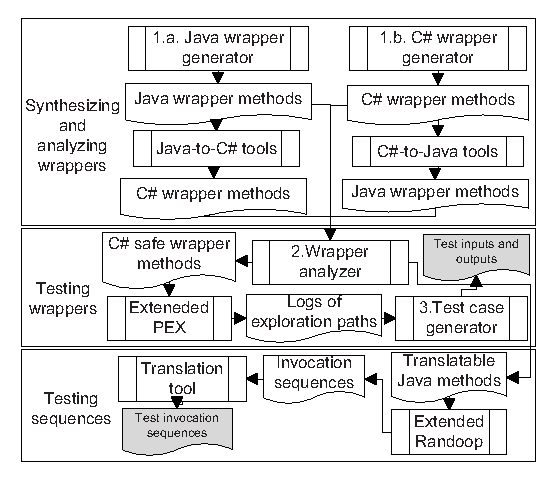
\includegraphics[scale=1,clip]{figure/approach.eps}\vspace*{-3ex}
 \caption{Overview of our approach}\vspace*{-3.5ex}
 \label{fig:approach}
\end{figure}

%-------------------------------------------------------------------
\subsection{Aligning Client Code}
\label{sec:approach:acc}

Initially, our approach accepts two versions of a project (one version in
$L_1$ and the other version in $L_2$) and aligns classes and methods
of the two versions. Aligned classes or methods
between the two versions implement a similar functionality. As they
implement a similar functionality, APIs used by these classes or methods can be
replaceable.

To align classes and methods of the two versions, our approach uses
name similarities between entities (such as class names or method names)
defined by the two versions of the project. In our approach, we have two
different kinds of entity names: entity names defined by the two versions
of the project and entity names of third-party libraries used by the two versions of the project.
The first kind often comes from the same programmer or the same team, or
programmers may refer to existing versions for naming entities such
as classes, methods, and variables. Therefore, name similarity is often
reliable to distinguish functionalities of the first kind compared to the second
kind. Our approach uses Simmetrics\footnote{\url{http://sourceforge.net/projects/simmetrics/}}
to calculate name similarities.

Algorithm 1 shows how our approach aligns client code classes. The
first step is to find candidate class pairs by names. For two sets
of classes ($C$ and $C'$), the algorithm returns candidate class
pairs ($M$) with a similarity greater than a given threshold,
referred to as \emph{SIM\_THRESHOLD}. As some projects may have many
classes with the same name, $M$ may contain more than one matching
pair for a class in a version. To align those classes, our algorithm
uses package names of these classes to refine $M$ and returns only
one matching pair with the maximum similarity\footnote{For C\#, we
refer to namespace names for package names.}.

In each aligned class pair, our approach further aligns methods
within the class pair. The algorithm for methods is similar to the
algorithm for classes but relies on other criteria such as the number of parameters
and names of parameters to refine candidate method pairs. These candidates
may contain more than one method pair due to overloading.
For the example shown in Section~\ref{sec:example}, our approach
correctly aligns the class \CodeIn{IndexFiles} and the method
\CodeIn{main} in Java to the class \CodeIn{IndexFiles}
and the method \CodeIn{Main} in C\# as their names are quite
similar.
%-----------------------------------------------------------------
\subsection{Mapping API classes}
\label{sec:approach:mappingtypes}

In this step, our approach mines mapping relations of
API classes. As defined in Section~\ref{sec:mapping}, mapping relations of API classes are used
to translate variables. Consequently, our approach mines mapping
relations of API classes based on how aligned client code declares
variables such as fields of aligned classes, parameters of aligned methods
and local variables of aligned methods. In
particular, for each aligned class pair $\Pair{c_1} {c_2}$, our
approach analyzes each field pair $\Pair{f_1}{f_2}$ and considers
$\Pair{f_1.type} {f_2.type}$ as one mined mapping relation of API
classes when the similarity between $f_1.name$ and $f_2.name$ is
greater than \emph{SIM\_THRESHOLD}. Similarly, for each aligned method pair
$\Pair{m_1} {m_2}$, our approach analyzes each local variable pair
$\Pair{var_1} {var_2}$ and considers $\langle var_1.type,$ $
var_2.type\rangle$ as one mined mapping relation of API classes when
the similarity between $var_1.name$ and $var_2.name$ is greater than
a threshold. Also, our approach analyzes each parameter pair
$\langle para_1, $ $para_2\rangle$ of $m_1$ and $m_2$, and our
approach considers $\langle para_1.type,$ $para_2.type\rangle$ as
one mined mapping relation of API classes when the similarity
between $para_1.name$ and $para_2.name$ is greater than \emph{SIM\_THRESHOLD}.

For the example shown in Section~\ref{sec:example}, our approach
mines the mapping relation between \CodeIn{java.io.File} and
\CodeIn{System.IO.FileInfo} based on the matched fields of Lines 4
and 9 (Figure~\ref{fig:clientcode}). The mapping relation of API classes helps translate the
variable declared in Line 1 (Figure~\ref{fig:totranslation})
to the variable declared in Line 16 (Figure~\ref{fig:translatedcode}).

%\begin{algorithm}[t]
%\begin{SmallOut}
%\dontprintsemicolon
%  \KwIn{$C$ is the classes of a language; $C'$ is the classes
%  of another language}
%  \KwOut{$P$ is aligned pairs of classes}
%  \Begin{
%     $M \leftarrow findCandidateClassPairs(C, C')$\;
%     \While{$M.size > 0 $}{
%        \If{$M.size > 1$}{
%            $M \leftarrow refineByPackageNames(M)$\;
%         }
%         \If{$M.size == 1$}{
%                $P.add(M)$\;
%                $C.remove(M[0].c)$\;
%                $C'.remove(M[0].c')$\;
%         }
%         $M \leftarrow findCandidateClassPairs(C, C')$\;
%     }
% }
%\end{SmallOut}
%\label{alg:alignclasses} \caption{Align Classes Algorithm}
%\end{algorithm}

\begin{figure}[t]
\centering
\includegraphics[scale=1,clip]{figure/algorithm1.eps}
\vspace*{-6ex}
\end{figure}

%-----------------------------------------------------------
\subsection{Mapping API methods}
\label{sec:approach:mappingtypes}

In this step, our approach mines mapping relations of API methods.
This step has two major sub-steps. First, our approach builds a graph, referred
as API transformation graph, for each client code
method. Second, our approach compares the two graphs of each paired
client code methods for mining mapping relations of API methods.

\begin{figure*}[t]
\centering
\includegraphics[scale=1.1,clip]{figure/graph.eps}\vspace*{-3ex}
 \caption
{\label{fig:graph}Built ATGs and the main steps of comparing
ATGs}\vspace*{-3.5ex}
\end{figure*}


\subsubsection{API transformation graph}
We propose API transformation graphs (ATG) to help deal with the two
challenges of mining API mapping listed in
Section~\ref{sec:introduction}. An API transformation graph of a
client code method $m$ is a directed graph
$G\Triple{N_{data}}{N_{m}}{E}$. $N_{data}$ is a set of the fields
$F$ of $m$'s declaring class, local variables $V$ of $m$, parameters
$P_1$ of $m$, parameters $P_2$ of methods called by $m$, and return
values $R$ of all methods. $N_{m}$ is a set of methods called by
$m$. $E$ is a set of directed edges. An edge $d_1\rightarrow d_2$
from a datum $d_1 \in N_{data}$ to a datum $d_2 \in N_{data}$
denotes the data dependency from $d_1$ to $d_2$. An edge $d_1
\rightarrow m_1$ from a datum $d_1 \in N_{data}$  to a method $ m_1
\in N_{m}$ denotes $d_1$ is a parameter or a related variable of
$m_1$. An edge $m_1 \rightarrow d_1$ from a method $m_1 \in N_{m}$
to a datum $d_1 \in N_{data}$ denotes $d_1$ is the return value of
$m_1$.

%We propose ATG for two main purposes. The first purpose is to mine mapping
%relations among parameters of mapped API methods. Mining mapping relations
%among parameters of mapped API methods is challenging as often mapped API methods
%can have different number of parameters or different positions among
%parameters. For example, consider the following two mapped API methods:
%
%\begin{CodeOut}
%$m_1$ in Java: BigDecimal java.math.BigDecimal.multiply (BigDecimal $p_1^1$)\\
%\hspace*{0.11in}$m_2$ in C\#: Decimal System.Decimal.Multiply (Decimal $p_1^2$, Decimal $p_2^2$)
%\end{CodeOut}
%
%Method $m_1$ of Java has a receiver variable, say $v_1^1$, of type \CodeIn{BigDecimal}
%and has one parameter $p_1^1$. The mapped method $m_2$ in C\# has
%two parameters $p_1^2$ and $p_2^2$. Using ATGs, our approach
%identifies that $v_1^1$ is mapped to $p_1^2$ and $p_1^1$ is mapped
%to $p_2^2$. As ATG captures parameters of API methods,
%our approach is able to deal with the challenges of mapping parameters.
%
%The second purpose of ATG is to mine mapping relations of merged API methods. As ATG
%describes data dependencies among inputs and outputs, our approach
%is able to mine mapping relations for merged API methods as shown in
%Figure~\ref{fig:example}. We next describe how our approach builds ATGs and
%uses ATGs for mining mapping relations of API methods.

\subsubsection{Building API transformation graphs }

Our approach builds an ATG for each method $m$. ATG includes information such as
inputs and outputs for each client code method. In particular, for
each method $m$, our approach first builds subgraph for its variables,
API methods, and field accesses according to the following rules:

%First, programming languages typically provide a huge set of APIs,
%and it is difficult to build mapping relations for all APIs
%manually. Second, some API methods have multiple parameters, and
%some parameters cannot be mapped directly one by one in orders. For
%example, \CodeIn{org.w3c.dom.Element.getAttributeNS()} and
%\CodeIn{System.Xml.XmlElement.GetAttribute()} both have two
%parameters, but the two parameters are inverse by their meanings.
%Third, one API method in one language may be mapped to more than one
%API method in other languages. For example, \CodeIn{java.util.
%LinkedList.removeLast()} returns the last value, and \CodeIn{System.
%Collections.Generic.LinkedList.RemoveLast()} does not return any
%values. To get that value, C\# programmers need to call more APIs,
%and thus one API method of Java is mapped to serval API methods of
%C\#.



%
%One challenge to mine mapping relations of two API methods lies in
%how to map their inputs correctly. Here, our approach both the
%receiver and the parameters of a method as the inputs of a
%method. Inputs of two API methods may be matched but are not in the
%same order. For example, as shown in Section~\ref{sec:example},
%\CodeIn{java.io. File.exist()} has a receiver whereas
%\CodeIn{System.IO.File.Exist()} has no receiver but a
%parameter. In addition, parameter orders may be quite different. For
%example, the parameter order of \CodeIn{org.w3c.
%dom.Element.getAttributeNS()} is inverse with the parameter order of
%\CodeIn{System.Xml.XmlElement.GetAttribute()}. To deal with the
%preceding problem,


\begin{enumerate}\vspace*{-2ex}
\item $\forall$ $f \in F \cup V \cup P_1$, our approach adds a node to the built ATG.
The reason for considering these variables such as fields in
declaring class or local variables in method $m$ used in client code
is that these variables are useful to analyze data dependencies
among API methods.\vspace*{-2ex}
%\begin{center}
%\includegraphics[scale=0.7,clip]{figure/rule1.eps}
%\end{center}
\item $\forall$ API methods of the form ``$T_0\ T.AM (T_1 p_1, \ldots, T_n p_n)$''
called by method $m$, our approach adds receiver (of type $T$) and
parameter nodes to the built ATG as shown below. Our approach does
not add receiver node for static API methods. \vspace*{-3ex}
\begin{center}
\includegraphics[scale=0.7,clip]{figure/rule2.eps}%\vspace*{-1.5ex}
\end{center}\vspace*{-3ex}
\item $\forall$ $f\in F \cup V$, if $f$ is a non-primitive variable
of type $T_1$ and a field $x$ of $T_1$ is accessed as $f.x$, our
approach adds nodes to the built ATG as shown below. As Java often
uses getters and setters whereas C\# often use field accesses, our
approach treats field accesses as a special type of method
calls.\vspace*{-2ex}
\begin{center}
\includegraphics[scale=0.7,clip]{figure/rule3.eps}%\vspace*{-1.5ex}
\end{center}\vspace*{-3ex}
\end{enumerate}

Our approach adds additional edges to the built ATG (and sub-graphs
inside ATG) representing data dependencies among built sub-graphs.
We use the following rules for adding additional edges to the built
ATG. \Comment{In particular, our approach analyzes source files of a
client code method statement by statement and adds edges according
to the rules as follows:} \vspace*{-1.5ex}
\begin{enumerate}
\item $\forall$ statements of the form $x = y$, where $x \in F \cup V \wedge y \in F \cup V$,
our approach adds an edge from $y$ to $x$. This edge represents that
$x$ is data dependent on $y$.\vspace*{-1.5ex}
\begin{center}
\includegraphics[scale=0.7,clip]{figure/rule4.eps}%\vspace*{-1.5ex}
\end{center}\vspace*{-1.5ex}
\item $\forall$ statements of the form $x = AM()$, where $x \in F \cup V$, our approach
adds an edge from $AM$ to $x$ if the return value of $AM$ is
assigned to $x$. This edge represents that $x$ is data dependent on
the return value of $AM$. \vspace*{-1.5ex}
\begin{center}
\includegraphics[scale=0.7,clip]{figure/rule5.eps}%\vspace*{-1.5ex}
\end{center}\vspace*{-1.5ex}
\item $\forall$ API methods $AM(x)$ called by method $m$, our approach
adds an edge from $x$ to the parameter node of $AM$. This edge
represents that the parameter of $AM$ is data dependent on
$x$.\vspace*{-1.5ex}
\begin{center}
\includegraphics[scale=0.7,clip]{figure/rule6.eps}%\vspace*{-1.5ex}
\end{center}\vspace*{-1.5ex}
\item $\forall$ statements of the form $m_2(m_1(x))$, our approach
adds an edge from the return value node of $m_1$ to the parameter
node of $m_2$ parameter node. This edge represents that the
parameter of $m_2$ is data dependent on the return value of
$m_1$.\vspace*{-1.5ex}
\begin{center}
\includegraphics[scale=0.7,clip]{figure/rule7.eps}%\vspace*{-1.5ex}
\end{center}\vspace*{-1.5ex}
\item $\forall$ statements of the form $x.m()$, our approach adds
an edge from $x$ to $m$ as $x$ is the receiver object of $m$. This
edge represents that the receiver object of $m$ is data dependent on
$x$.\vspace*{-1.5ex}
\begin{center}
\includegraphics[scale=0.7,clip]{figure/rule8.eps}%\vspace*{-1.5ex}
\end{center}\vspace*{-1.5ex}
\item $\forall$ statements of the form $ x = y\ op\ z\ op\ \ldots, op \in \{+,-,*,/\}$,
our approach adds edges from $y$, $z$, and others to $x$, as these
variables are connected by binary operations and the return value is
assigned to $x$. The edge denotes the data dependency from $y$, $z$,
and other variables to $x$. For simplicity, our approach ignores
\emph{op} info. We discuss the issue in
Section~\ref{sec:discuss}.\vspace*{-1.5ex}
\begin{center}
\includegraphics[scale=0.7,clip]{figure/rule9.eps}%\vspace*{-1.5ex}
\end{center}\vspace*{-2ex}
\end{enumerate}

For each method $m$ in the client code, our approach applies preceding
rules for each statement from the beginning to the end of $m$.
Within each statement, our approach applies these rules based on
their nesting depth in the abstract syntax tree. For example,
for the statements of the form $m_2(m_1(x))$, our approach first applies
these rules on $m_1$ and then on $m_2$.

Figures~\ref{fig:graph}a and ~\ref{fig:graph}b show partial ATGs for
C\# (\CodeIn{IndexFiles.cs}) and Java (\CodeIn{IndexFiles.java})
code examples shown in Figure~\ref{fig:clientcode}, respectively.
Figure~\ref{fig:graph} also shows corresponding line numbers of each
sub-graph. Our approach applies Rules 2 and 6 for Lines 4 and 9 (Figure~\ref{fig:clientcode})
to build corresponding sub-graphs in the ATG. For
Lines 6 and 7 (Figure~\ref{fig:clientcode}), our approach applies Rules 2 and 8 to build
corresponding sub-graphs in the ATG. For Lines 12 and 15 (Figure~\ref{fig:clientcode}),
our approach applies Rule 2, 3, and 6 to build corresponding sub-graphs.

%\begin{algorithm}[t]
%\begin{SmallOut}
%\label{alg:mapATG} \dontprintsemicolon
%  \KwIn{$G$ is the ATG of a method ($m$); $G'$ is the ATG of $m$'s mapped method.}
%  \KwOut{$S$ is a set of mapping relations for API methods}
%  \Begin{
%     $P \leftarrow findVarPairs(m, m')$\;
%     \For{Pair p in P}{
%        $SM \leftarrow G.nextMethods(p.sharp)$\;
%        $JM \leftarrow G.nextMethods(p.java)$\;
%        $\Delta S = mapping(SM, JM)$\;
%        \While{$\Delta S \neq \phi| \Delta SM \neq \phi| \Delta JM \neq \phi$}{
%            $S.addAll(\Delta S)$\;
%             \For{Method sm in SM}{
%                 \If{$sm.isMapped$}{
%                    $SM.replace(sm, sm.nextMethod())$\;
%                  }\Else{
%                    $SM.replace(sm, sm.mergeNextMethod())$\;
%                  }
%             }
%             \For{Method jm in JM}{
%                 \If{$jm.isMapped$}{
%                    $JM.replace(jm, jm.nextMethod())$\;
%                  }\Else{
%                    $JM.replace(jm, Jm.mergeNextMethod())$\;
%                  }
%             }
%             $\Delta S = mapping(SM, JM)$\;
%        }
%     }
% }
% \end{SmallOut}
%\caption{ATG Comparison Algorithm}
%\end{algorithm}

\begin{figure}[t]
\centering
\includegraphics[scale=1,clip]{figure/algorithm2.eps}
\vspace*{-6ex}
\end{figure}

%--------------------------------------------------------------------
\subsubsection{Comparing API transformation graphs}

The second sub-step compares each pair of built ATGs for mining mapping
relations of API methods. Our mapped API methods satisfy three
criteria: (1) Mapped API methods implement the same
functionality. (2) Mapping relation describes the relation
between parameters of mapped API methods. (3) Mapping relation
describes the relation between return values of
mapped API methods. The two mapped API methods in two
different languages satisfying the preceding three criteria
are replaceable in the client code. Therefore, these mapped API
methods assist for migrating client code from one language to another.

Algorithm 2 presents major steps of comparing ATGs for mining
mapping relations of API methods. Consider two methods $m$ and $m'$
of two different languages $L$ and $L'$, respectively, in the client
code. Consider that the associated ATGs of $m$ and $m'$ are compared
to mine mapping relations of API methods. First, our algorithm finds
matching variables $\in$ $F$, $V$, and $P_1$ in $m$ and $m'$. Our
algorithm maps two variables $v$ and $v'$ of methods $m$ and $m'$,
respectively, if the similarity measure on their names is greater
than \emph{SIM\_THRESHOLD}. For constants in $m$ and $m'$, our
algorithm maps those two constants, if they have exactly the same
value. Our algorithm uses these variable and constant mappings to
compute mappings between API methods that use these variables and
constants. Our algorithm uses the following criteria for mapping two
API methods $jm$ and $sm$.

\emph{Matching entities}: The first criterion is based on entities such as receiver variable
or parameters of $jm$ and $sm$ to map $jm$ and $sm$. We map $jm$ with $sm$, if
the receiver variable of API method $jm$ is mapped
to the receiver variable of $sm$, and there is a one-to-one mapping between parameters
of $jm$ and $sm$.

\emph{Matching functionalities}: The second criterion is based on functionalities of
$jm$ and $sm$. We consider that $jm$ and $sm$ implement the same functionality,
if the similarity measure between the name of $jm$ and the name of $sm$ is
greater than \emph{SIM\_THRESHOLD}.

\emph{Matching outputs:} The third criterion is based on the return values of $jm$ and $sm$.
Consider the return values of $jm$ and $sm$ as $r_1$ and $r_2$, respectively. We map $jm$
with $sm$, if the type of $r_1$ is mapped with the type of $r_2$ in mapping API classes
relationship.

Our algorithm first attempts to map first API method $jm$ in $m$
with the first API method $sm$ in $m'$. If our algorithm successfully maps $jm$ with
$sm$, our algorithm moves to the next available API methods in $m$
and $m'$ of the client code. If our algorithm does not able to map $jm$
with $sm$, our algorithm merges $sm$ and $jm$ with their next available API methods
in the corresponding ATGs, respectively, and attempts to map merged API methods.
For two merged API methods, our algorithm uses the
maximum similarity of method names between $jm$ and $sm$ as a
similarity measure for matching their functionalities.
With each iteration, $sm$ or $jm$ or the mapping relation (represented as $S$)
in the algorithm changes. Therefore, we repeat our algorithm
till $S$, $sm$, and $jm$ do not change anymore.

We next explain our algorithm using the illustrative example shown
in Figure~\ref{fig:graph}. The numbers shown in circles
represent the major steps in our algorithm for mining mapping
relations of API methods. We next explain each step in detail.

\emph{S1: mapping parameters, fields, local variables, and constants.}
Given two ATGs of each method pair $\langle m, m' \rangle$, this step maps
variables such as parameters, fields, and local variables by comparing their names
and maps constants by comparing their values. As shown in
Figure~\ref{fig:graph}, Step 1 maps two constants as both the constants
have the same value \CodeIn{index}.

\emph{S2: mapping inputs of API methods.} Step 2 mines mapping
relations of API methods using variable and constant mapping relations.
Initially, this step identifies first API methods in the two ATGs and tries to
map their parameters and receiver objects of the two API methods.
In our current example, this step maps the parameter \CodeIn{filename}
to the parameter \CodeIn{arg0} as these parameters
are of the same type and their associated constants are mapped.

\emph{S3: mapping outputs of API methods.} In contrast to Step 2
that maps parameters, Step 3 maps return values of API methods. In
this step, if our approach is not able to map return values, our
approach merges the next API method and then attempts to map return
values of merged API methods. In our current example shown in
Figure~\ref{fig:graph}, return value of
\CodeIn{System.IO.FileInfo.FileInfo()} cannot be mapped to the
return value of \CodeIn{java.io.File.File()}. Therefore, our
approach merges next API methods in the ATG till the \CodeIn{Exists}
API method, as the return values (shown as \CodeIn{Boolean}) match
only after the \CodeIn{Exists} API method. Figure~\ref{fig:graph}
shows Step 3 along with the matching return values.

\emph{S4: mapping functionalities.} After our approach maps parameters and return values,
this step further maps functionalities of those merged API
methods. Given two merged API methods with mapped parameters and return values,
this step uses the similarity measure based of their method names as a criterion
for matching their functionalities. In the preceding example, this step maps
the two merged API methods shown in Figure~\ref{fig:graph}a to the
merged API methods of the \CodeIn{java.io.File.exist()} as all three
merged API methods include the method named \CodeIn{exist}.

Our approach applies preceding steps on ATGs
(as shown in Figures~\ref{fig:graph}a and~\ref{fig:graph}b) and mines
mapping relations. An example mapping relation from the preceding ATGs is
shown in Figure~\ref{fig:example}.


\section{Evaluations}
\label{sec:eval}

We conducted three evaluations to show the effectiveness of our approach in generating regression tests that achieve a high coverage of the code under test. Our empirical results show that our approach is scalable and can automatically generate tests for large real-word applications without any manual efforts. In our evaluations,  we use two core .NET 2.0 framework libraries\footnote{\url{http://msdn.microsoft.com/en-us/library/ms229335.aspx}} as subject applications. We next describe the research questions addressed in our evaluation and present our evaluation results.

%\begin{figure*}[t]
%\centering
%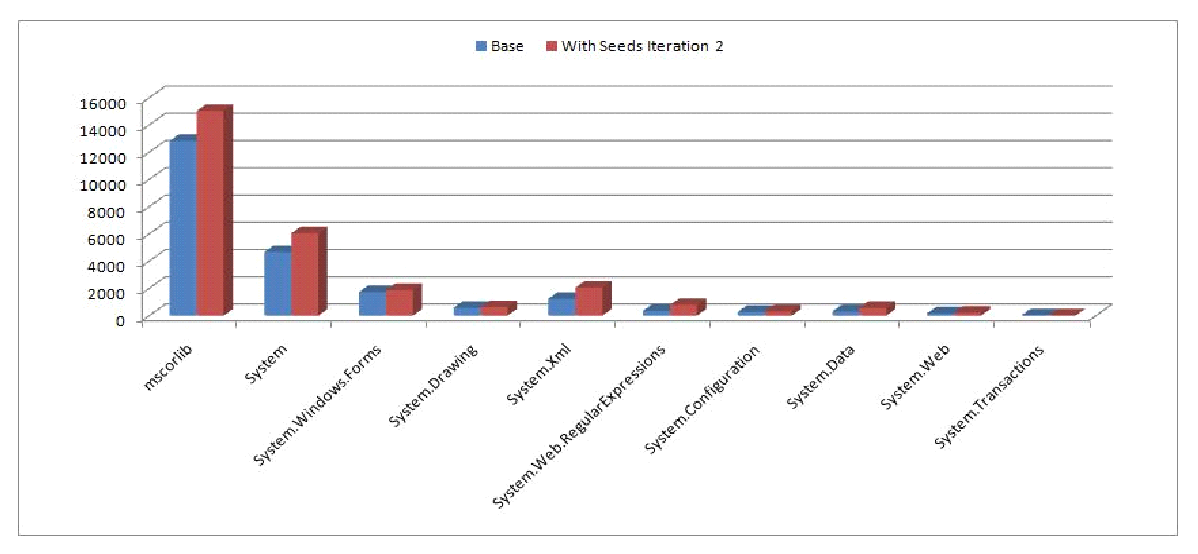
\includegraphics[scale=0.70,clip]{figs/RQ2_1.eps}\vspace*{-1ex}
%\caption{Comparison of base coverage and coverage achieved by regression tests of Mode 4 (WithSeeds Iteration 2).} \label{fig:rq2}
%\end{figure*}

%---------------------------------------------------------------------------------------
\subsection{Research Questions}
\label{sec:research}

We address the following three research questions in our evaluations.

\begin{itemize}
\item RQ1: Can our approach handle large real-world applications in automatically generating regression tests that achieve a high coverage of the code under test? 
\item RQ2: Do seed tests help achieve higher coverage of the code under test than without using seed tests?
\item RQ3: Can more machine power help generate new regression tests that can achieve more coverage of the code under test?
\end{itemize}

%---------------------------------------------------------------------------------------
\subsection{Subject Applications}

We used two core .NET 2.0 framework base class libraries as subject applications in our evaluations. We selected these libraries because these libraries are shipped and maintained in different distributions such as Version 2 and Version 4 of the ``desktop CLR'', 32-bit/64-bit Silverlight, and .NET compact framework. Therefore, it is paramount for the .NET product group to maintain identical behavior and detect any new defects between different versions of these base class libraries. Table~\ref{tab:subjects} shows the two libraries (mscorlib and System) used in our evaluations and their characteristics such as the number of classes and methods. The table also shows statistics of eight other libraries of .NET 2.0 framework. Although these other eight libraries are not our primary targets for generating regression tests, our generated regression tests include methods from these libraries since these libraries are developed based on the two core libraries: mscorlib and System. In our evaluations, we use these additional eight libraries also while presenting our coverage results. The table shows that these libraries include $0$ LOC with $0$ classes and $0$ methods.

\setlength{\tabcolsep}{1pt}
\begin{table}[t]
\begin{SmallOut}
\begin{CodeOut}
\begin{center}
\begin {tabular} {|l|c|c|c|}
\hline
\textbf{.NET libraries} & \textbf{LOC} & \textbf{\# public} & \textbf{\# public}\\ 
 & & \textbf{classes} & \textbf{methods}\\ 
\hline
\hline  mscorlib & 185K & 1440 & 17800 \\
\hline  System & & & \\
\hline  System.Windows.Forms & & & \\
\hline  System.Drawing & & & \\
\hline  System.Xml & 150K & 686 & 9920 \\
\hline  System.Web.RegularExpressions & & & \\
\hline  System.Configuration & & & \\
\hline  System.Data & 196K & 648 & 11550 \\
\hline  System.Web &  & & \\
\hline  System.Transactions & & & \\
\hline \textbf{TOTAL} &  &  &   \\
\hline
\end{tabular}
\end{center}
\end{CodeOut}
\end{SmallOut}\vspace*{-4ex}
\centering \caption {\label{tab:subjects}Ten .NET framework base class libraries used in our evaluations}
\end{table}

%---------------------------------------------------------------------------------------
\subsection{Evaluation Setup}

In our approach, we used nine machines that can be classified into three configuration categories. On each machine, we launched multiple Pex processes. The number of processes launched on a machine is based on the configuration of the machine. For example, on an eight core machine, we launched seven Pex processes. Each Pex process was exploring one class (including multiple PUTs) at a time. Table~\ref{tab:mconfig} shows all three configuration categories. The table also shows the number of machines of each configuration and the number of Pex processes launched on each machine.

\setlength{\tabcolsep}{1pt}
\begin{table}[t]
\begin{SmallOut}
\begin{CodeOut}
\begin{center}
\begin {tabular} {|l|c|c|}
\hline
\textbf{Machine Configuration} & \textbf{\# of} & \textbf{\# of} \\  
 & \textbf{machines} & \textbf{processes}\\  
\hline
\hline  Xeon 2 CPU @ 2.50 GHz, 8 cores & 1 & 7\\
				16 GB RAM & & \\
\hline  Quad core 2 CPU @ 1.90 GHz, 8 cores& 2 & 7\\
				8 GB RAM & & \\
\hline  Intel Xeon CPU @2.40 GHz, 2 cores& 6 & 1\\
				1 GB RAM & & \\
\hline
\end{tabular}
\end{center}
\end{CodeOut}
\end{SmallOut}\vspace*{-4ex}
\centering \caption {\label{tab:mconfig}Three categories of machine configurations used in our evaluations.}
\end{table}

As we used .NET framework base class libraries in our evaluations, the generated tests may invoke method calls that can can cause external side effects, and change the machine configuration. Therefore, while executing the code during exploration of PUTs or while running generated tests, we created a sand-box with the ``Internet'' security permission. This permission represents the default policy permission set for the content from an unknown origin. This permission blocks all operations that involve environment interactions such as file creations or registry accesses by throwing \CodeIn{SecurityException}. Since we use sand-box in our evaluations, the reported coverage is lower than the actual coverage that can be achieved by our generated regression tests.

To address our research questions, we first created a base line in terms of the code coverage achieved by the seed tests, referred to as \emph{base coverage}. In our evaluations, we use block coverage (Section~\ref{sec:blockcov}) as a coverage criteria. We report our coverage in terms of the number of blocks covered in the code under test. We don't give an upper bound on the number of reachable basic blocks, as we don't know which blocks are actually reachable from the given scenarios.

We next generated regression tests in four different modes. In Mode 1 (referred to as \emph{WithoutSeeds Iteration 1}), we generated regression tests without using seed tests for one iteration. In Mode 2 (referred to as \emph{WithoutSeeds Iteration 2}), we generated regression tests without using seed tests for two iterations. The regression tests generated in Mode 2 are a super set of the regression tests generated in Mode 1. In Mode 3 (referred to as \emph{WithSeeds Iteration 1}), we generated regression tests with using seed tests for one iteration. Finally, in Mode 4 (referred to as \emph{WithSeeds Iteration 2}), we generated regression tests with using seed tests for two iterations. Modes 1 and 3 took one and half day for generating tests, whereas Modes 2 and 4 took three days since these modes correspond to Iteration 2.

\setlength{\tabcolsep}{1pt}
\begin{table}[t]
\begin{SmallOut}
\begin{CodeOut}
\begin{center}
\begin {tabular} {|l|c|c|c|}
\hline
\textbf{Mode} & \textbf{\# of} & \textbf{\# of covered} & \textbf{\% of increase}\\  
 & \textbf{Tests} & \textbf{blocks} & \textbf{from base}\\  
\hline
\hline  WithoutSeeds Iteration 1 & 248,306 & 21,920 & 0\%\\
\hline  WithoutSeeds Iteration 2 & 412,928 & 23,176 & 4.8\%\\
\hline  WithSeeds Iteration 1 & 376,367 & 26,939 & 21.8\%\\
\hline  WithSeeds Iteration 2 & 501,799 & 27,485 & 24.3\%\\
\hline
\end{tabular}
\end{center}
\end{CodeOut}
\end{SmallOut}\vspace*{-4ex}
\centering \caption {\label{tab:gentests}Generated regression tests.}
\end{table}

%---------------------------------------------------------------------------------------
\subsection{RQ1: Generated Regression Tests}

We next address the first research question of whether our approach can handle large real-world applications in automatically generating regression tests. This research question helps to show that our approach can be used in practice and can address scalability issues in generating regression tests for large applications. We first present the statistics after each phase in our approach and next present the number of regression tests generated in each mode.

In the capture phase, our approach recorded $\approx$1.50 GB C\# source code (including 433,809 traces) of dynamic traces for the two libraries. The average trace length includes $21$ method calls and the maximum trace length includes $52$ method calls. As our capture phase transforms each dynamic trace into a PUT and a seed test, the capture phase resulted in 433,809 PUTs and 433,809 seed tests. 

In the minimize phase, our approach uses static analysis to filter out duplicate PUTs. Our static analysis took 45 minutes and resulted in 68,575 unique PUTs. Our approach uses dynamic analysis to filter our duplicate seed tests. Our dynamic analysis took 5 hours and resulted in 128,185 unique seed tests. These results show that there are a large number of duplicate PUTs and seed tests, and show the significance of our minimize phase. We next measured the block coverage achieved by these 128,185 unique seed tests in the code under test and used this coverage as \emph{base coverage}. These tests covered 22,111 blocks in the code under test. 

Table~\ref{tab:gentests} shows the number of regression tests generated in each mode along with the number of covered blocks. The table also shows the percentage of increase
in the number of blocks compared to the base coverage. As shown in results, in Mode 4 (WithSeeds Iteration 2), our approach achieved 24.3\% higher coverage than the base coverage. Table~\ref{tab:detailedres} shows more detailed results of coverages achieved for all ten .NET libraries. Column ``.NET libraries'' shows the library under test. Column ``Base Coverage'' shows the number of blocks covered by seed tests for each library. Column ``WithOutSeeds Iteration 1'' shows the number of blocks covered (``\# blocks'') and the percentage of increase in the coverage (``\% increase'') with respect to the base coverage in this mode. Similarly, Columns ``WithOutSeeds Iteration 2'', ``WithSeeds Iteration 1'', and ``WithSeeds Iteration 2'' show the results of the other three modes. 

As we use seed tests during our exploration in Mode ``WithSeeds Iteration 2'', the coverage achieved is either the same or higher than the base coverage. However, our approach has achieved significant higher coverages than base coverage for libraries mscorlib and System (in terms of the number of additional blocks covered). The primary reason is that most of the classes in these libraries are stateless and do not require environment interactions. The results show that our approach can handle large real-world applications and can generate large number of regression tests that achieve a high coverage of the code under test.

\setlength{\tabcolsep}{1pt}
\begin{table*}[t]
\begin{SmallOut}
\begin{CodeOut}
\begin{center}
\begin {tabular} {|l|c|c|c|c|c|c|c|c|c|}
\hline
\textbf{.NET libraries} & \textbf{Base} & \multicolumn{2}{|c|}{\textbf{WithOutSeeds}} & \multicolumn{2}{|c|}{\textbf{WithOutSeeds}} & \multicolumn{2}{|c|}{\textbf{WithSeeds}} & \multicolumn{2}{|c|}{\textbf{WithSeeds}}\\ 
 & \textbf{Coverage} & \multicolumn{2}{|c|}{\textbf{Iteration 1}} & \multicolumn{2}{|c|}{\textbf{Iteration 2}} & \multicolumn{2}{|c|}{\textbf{Iteration 1}} & \multicolumn{2}{|c|}{\textbf{Iteration 2}}\\ 
\cline{3-10}
 & \# blocks & \# blocks & \% increase & \# blocks & \% increase & \# blocks & \% increase & \# blocks & \% increase\\ 
\hline  mscorlib   						& 12827 	& 13063 & 1.84		& 13620 & 6.18	& 14808	& 15.44		& 15018	& 17.08					\\
\hline  System    						& 4651  	& 4062  & -12.67	& 4243	& -8.77	& 5907	& 27.00		& 6039	& 29.84 				\\
\hline  System.Windows.Forms  & 1730 		& 1572  & -9.13		& 1774	& 2.54	& 1782	& 3.01		& 1865	& 7.80 					\\
\hline  System.Drawing 				& 570			& 580		& 1.75		& 591		& 3.68	& 618		& 8.42		& 625		& 9.65 					\\
\hline  System.Xml 						& 1229    & 1390	& 13.10		& 1462	& 18.96	& 1959	& 59.40		& 2045	& 66.40 				\\
\hline  System.Web.Regular 		& 351     & 330		& -5.98		& 520		& 48.15	& 754		& 114.81 	& 771		& 119.66 				\\
			  Expressions 					& 				& 			& 				& 			& 			& 			& 				& 			&  							\\
\hline  System.Configuration 	& 263 		& 297 	& 12.93		& 297		& 12.93	& 302		& 14.83		& 306		& 16.35 				\\
\hline  System.Data 					& 301 		& 380		& 26.25		& 422		& 40.20	& 562		& 86.71		& 569		& 89.04 				\\
\hline  System.Web 						& 154			& 211		& 37.01		& 212		& 37.66	& 212		& 37.66		& 212		& 37.66 				\\
\hline  System.Transactions 	& 35			& 35		& 0.00		& 35		& 0.00	& 35		& 0.00		& 35		& 0.00 					\\
\hline \textbf{TOTAL/AVERAGE} & \textbf{22111} & \textbf{21920} & \textbf{<0} & \textbf{23176} & \textbf{4.80} & \textbf{26939}	& \textbf{21.80} & \textbf{27485} & \textbf{24.30} \\
\hline
\end{tabular}
\end{center}
\end{CodeOut}
\end{SmallOut}
\centering \caption {\label{tab:detailedres}Comparison of coverages achieved for ten .NET libraries used in our evaluation.}
\end{table*}

%---------------------------------------------------------------------------------------
\subsection{RQ2: Using Seed Tests}

We next address the second research question of whether seed tests help achieve higher code coverage compared to without using seed tests. To address this question, we compare the coverages achieved by generated tests in Modes ``WithoutSeeds Iteration 2'' and ``WithSeeds Iteration 2''. As shown in Table~\ref{tab:detailedres}, Mode ``WithSeeds Iteration 2'' always achieved higher coverage than Mode ``WithoutSeeds Iteration 2''. On average ``WithSeeds Iteration 2'' achieved 18.6\% higher coverage than Mode ``WithoutSeeds Iteration 2''. The table also shows that there is a significant increase in the coverage achieved for the \CodeIn{System.Web.RegularExpressions} library. 
In Section~\ref{sec:explore}, we described one of the advantages of seed tests is that seed tests can help cover certain paths that are hard to be covered without using those tests. The \CodeIn{System.Web.RegularExpressions} library is an example for such paths since this library requires complex regular expressions to cover certain paths in the library. It is quite challenging for Pex or any other dynamic-symbolic-execution-based approach to generate concrete values that represent regular expressions. Therefore, concrete values in the seed tests helped achieve higher coverage for this library. In summary, the results show that seed tests help achieve higher coverages compared to without using seed tests.

%\begin{figure*}[t]
%\centering
%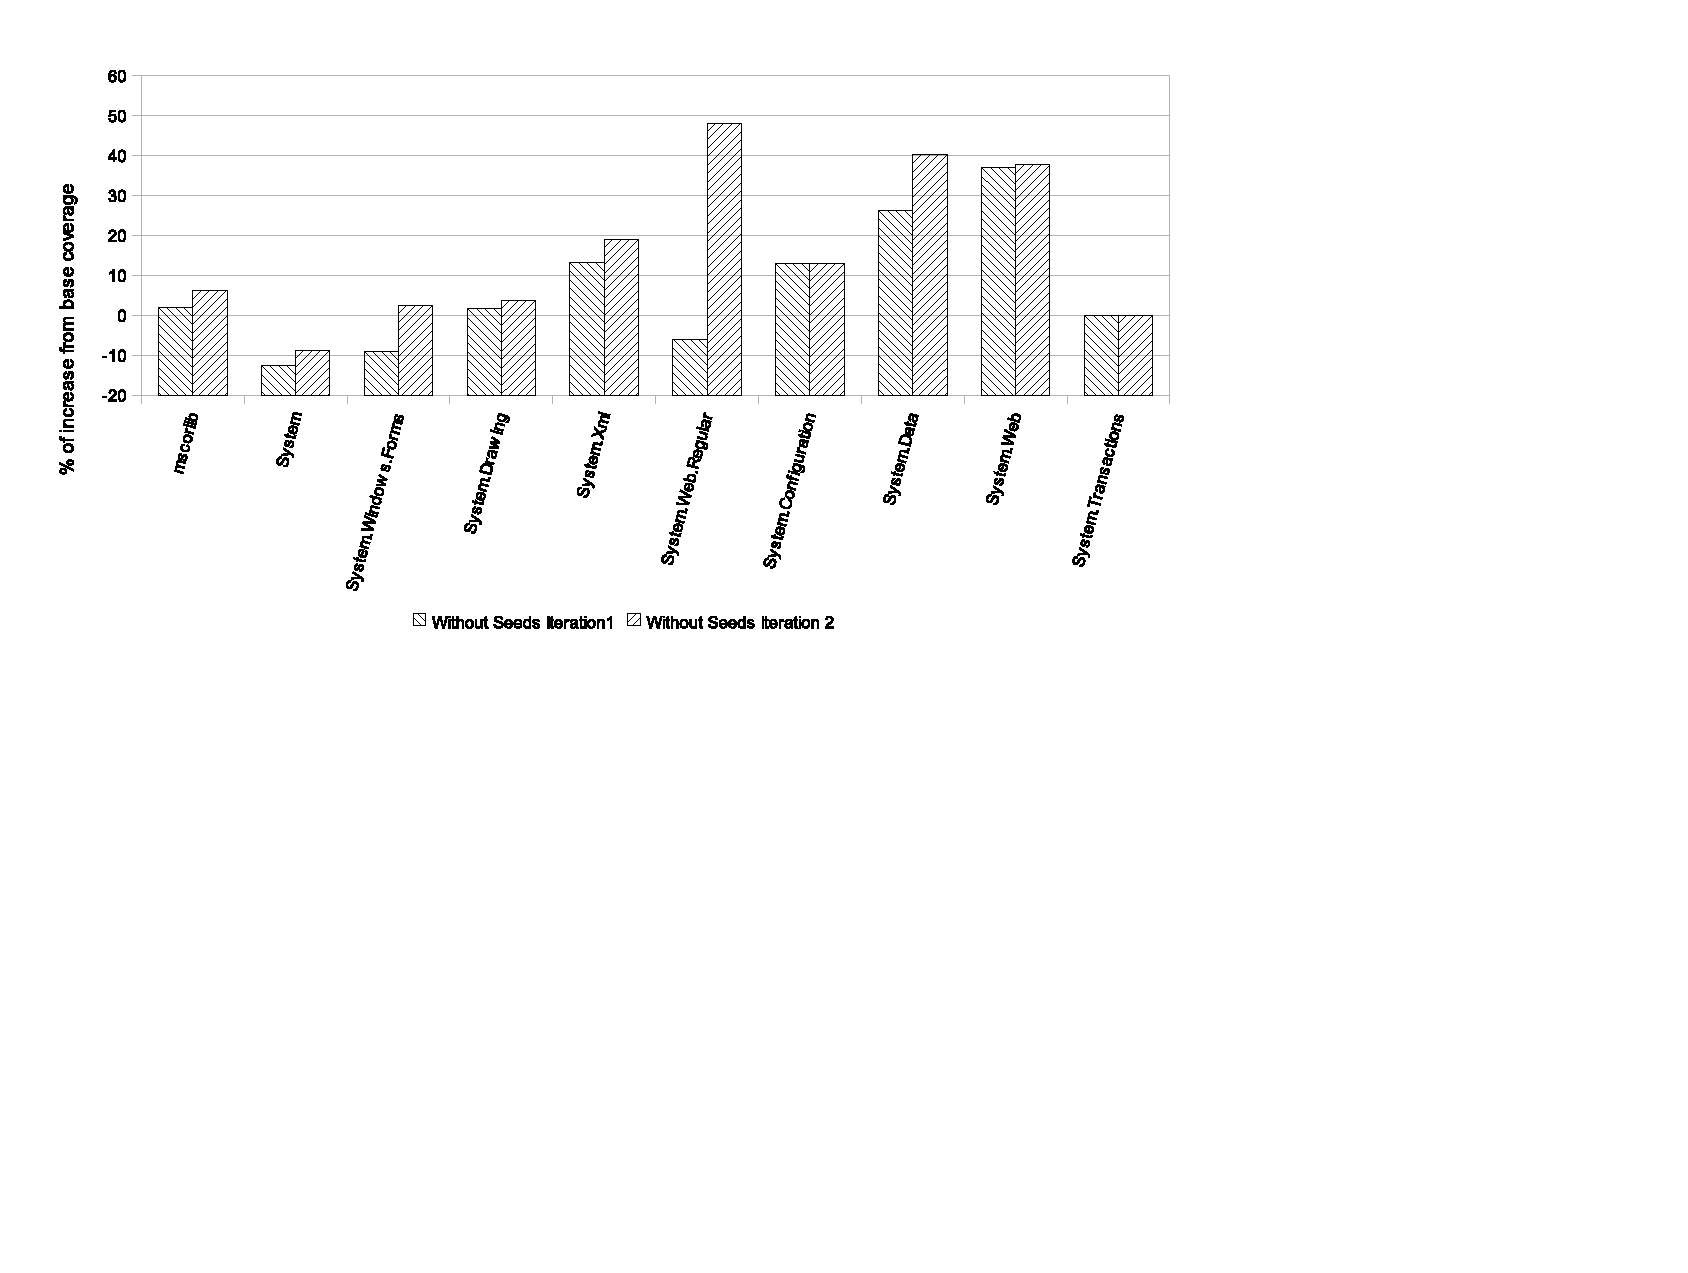
\includegraphics[scale=0.70,clip]{figs/RQ3_1.eps}\vspace*{-1ex}
%\caption{Comparison of code coverages achieved by base, Modes 2 (WithoutSeeds Iteration 2) and 4 (Withseeds Iteration 2).} \label{fig:rq3}
%\end{figure*}

%---------------------------------------------------------------------------------------
\subsection{RQ3: Using More Machine Power}

We next address the third research question of whether more machine power helps to achieve more coverage. This research question helps to show that additional coverage can be achieved in further iterations of our approach. To address this question, we compare coverages achieved in Mode ``WithoutSeeds Iteration 1'' with Mode ``WithoutSeeds Iteration 2'', and Mode ``WithSeeds Iteration 2'' with Mode ``WithSeeds Iteration 2'' (shown in Table~\ref{tab:detailedres}). 

On average, Mode ``WithoutSeeds Iteration 2'' achieved 5.73\% higher coverage than Mode 1. This result show that our approach can achieve additional coverage in further iterations. However, the coverage from Mode 1 to Mode 2 is not doubled. The primary reason is that it gets harder to cover new blocks in further iterations.

Figure~\ref{fig:rq42} shows the comparison results of Mode 3 with Mode 4. On average, Mode 4 achieved 2.0\% higher coverage than Mode 3. As shown, the increase in coverage from Mode 3 to Mode 4 is less than the increase in the coverage from Mode 1 to Mode 2. This difference is due to seed tests that help achieve higher coverage during Mode 3, leaving more harder blocks to be covered in Mode 4. In summary, the results show that further iterations can help generate new regression tests that can achieve more coverage.

\begin{figure*}[t]
\centering
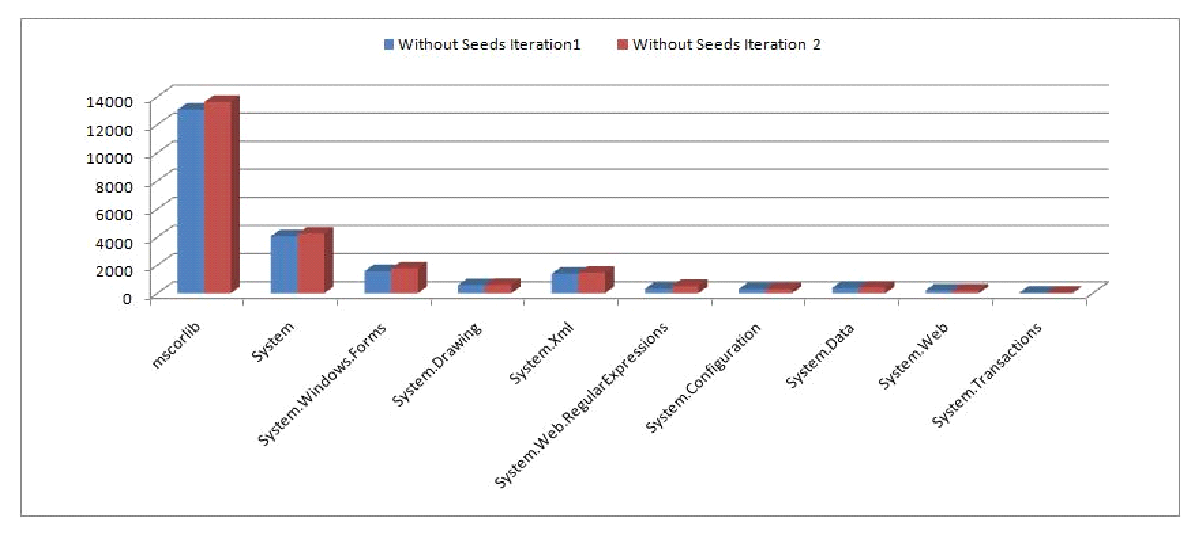
\includegraphics[scale=0.70,clip]{figs/RQ4_1_1.eps}\vspace*{-1ex}
\caption{\label{fig:rq41}Comparison of code coverages achieved by Modes 1 (WithoutSeeds Iteration 1) and 2 (WithoutSeeds Iteration 2).} 
\end{figure*}


\begin{figure*}[t]
\centering
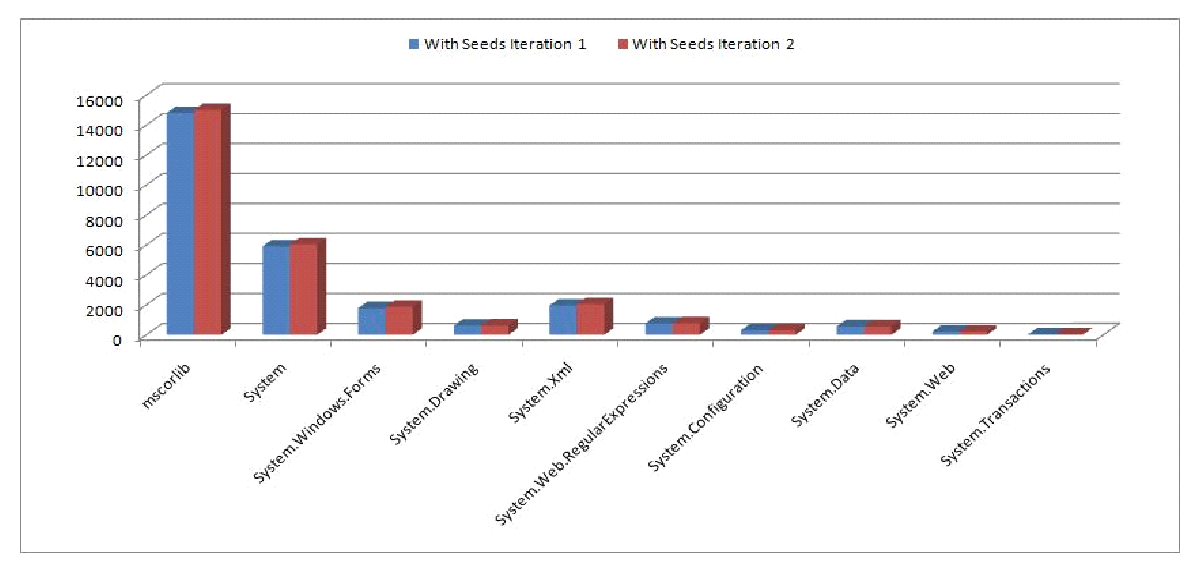
\includegraphics[scale=0.70,clip]{figs/RQ4_2_1.eps}\vspace*{-1ex}
\caption{\label{fig:rq42}Comparison of code coverages achieved by Modes 3 (WithSeeds Iteration 1) and 4 (Withseeds Iteration 2).}
\end{figure*}


%---------------------------------------------------------------------------------------
%\subsection{Real Defects}

%Our approach automatically generates test scenarios from dynamic traces. We use these test scenarios
%in generating PUTs and then generating regression tests on a stable versions. These regression tests
%can be used on future versions to detect regression faults. In our approach, we cannot detect
%defects in the version on which regression tests generated because of lack of test oracles. However,
%we identify that many exceptions are observed while generating regression tests on the version.
%We next describe the raised exceptions and describe more about the defects detected.

\section{Threats to Validity}
\label{sec:threats}
The threats to external validity primarily include the degree to which the subject programs and used CSE are representative of true practice. The current subjects range from small-scale libraries such as Java SQL APIs to large-scale libraries such as BCEL and Hibernate. We used only one CSE, i.e., Google code search, which is a well-known CSE. These threats could be reduced by more experiments on wider types of subjects and by using other CSEs in future work. The threats to internal validity are instrumentation effects that can bias our results. Faults in our Alattin prototype might cause such effects. There can be errors in our inspection of source code for confirming rules or defects. To reduce these threats, we inspected available specifications and also call sites in source code.

\section{Discussion and Future Work}
\label{sec:discuss} In this section, we discuss related issues of
our approach.

\textbf{Aligning client code of similar functionalities.} As shown
in Table~\ref{table:analyzingclient}, our approach sometimes fails
to align client code. For some considerations, programmers may
implement one functionality as one class or one method in one
language version but implement the same functionality as multiple
classes or methods in another language version. One feasible way to
align these functionalities is to analyze them dynamically. For
example, Jiang and Su~\cite{jiang2009automatic} propose an approach
to mine code snippets of similar functionalities. We plan to develop
a dynamic technique for those unmatched classes or methods in our
future work.
\begin{figure}[t]
\centering
\includegraphics[scale=1,clip]{figure/n2n.eps}\vspace*{-3ex}
 \caption{Merging technique}\vspace*{-3.5ex}
 \label{fig:n2n}
\end{figure}

\textbf{Mining richer API mapping.} As shown in
Table~\ref{table:compare}, although we use 10 large projects as
subjects, our evaluation does not achieve high recalls for J2SE. For
a given library, these projects still do not provide adequate source
files for mining. Our previous
work~\cite{thummalapenta07parseweb,thummalapentaase08spotweb} shows
that it is feasible to use the internet-scale open source code
available on the web as subjects for mining with the help of code
search engines such as Google code
search\footnote{\url{http://www.google.com/codesearch}}. We plan to
leverage those search engines to mine richer API mapping in our
future work.

\textbf{Ranking mined mapping relations.} One API class or method
can be mapped to more than one class or method. When comparing with
CSharp2Java, we choose the formal as the generated mapping files
since the support of the former is 46 whereas the support of the
latter is 4. However, in some cases, the API mapping with the
highest support is not necessarily the best choice. For example,
\CodeIn{java.util.ArrayList} is mapped to
\CodeIn{System.Collections.ArrayList} based on support values. The
Java class supports generic programming, whereas the C\# class does
not. Consequently, the Java class seems to be better mapped to
\CodeIn{System.Collections.Generic.List} as this C\# class also
supports generic programming. We plan to develop ranking techniques
to address this issue in future work.

\textbf{Mining more many-to-many mapping relations of API methods.}
A majority of mined mapping relations of API methods describe
one-to-one relations. Algorithm 2 merges the next API method with a
forward strategy. For the example shown in Figure~\ref{fig:n2n}, if
the algorithm merges \CodeIn{method1()} and \CodeIn{method2()} but
fails to find a match, the algorithm tries to merge
\CodeIn{method3()}. In some cases, a match can be found if the
algorithm merges \CodeIn{method4()} instead of \CodeIn{method3()}.
We plan to improve the algorithm to mine more many-to-many relations
in future work.

\textbf{Migrating many-to-many mapping relations of API methods.} A
mined many-to-many mapping of API methods may have multiple outputs
and complicated internal data processes. Our defined API
transformation graphs help find out all essential API methods.
However a graph does not describe adequate details to support
automatic translation. For example, we need to manually add an
\emph{or} operator for the two outputs of the API mapping shown in
Figure~\ref{fig:example}. We plan to add more details to help
automate migration with many-to-many mapping relations in future
work.

\textbf{Migrating unmapped APIs.} Our approach mines API mapping of
methods that have mapped inputs, mapped outputs, and similar
functionalities. Consequently, mined API mapping can be migrated
automatically. However, some APIs between two languages cannot
satisfy all the three criteria. For these APIs, if outputs are
unmapped, our approach can simply ignore outputs when outputs are
not used in client code. If inputs or functionalities are unmapped,
we plan to develop techniques that analyze how two versions of a
project deal with a similar unmapped API problem for some reusable
code snippets in future work.


\section{Related Work}
\label{sec:related} In this section, we introduce related work and
discuss our contributions.

\textbf{Language migration.} It is a research topic with a long
history to migrate projects of one language into other
languages~\cite{samet1981experience}. To reduce the human effort of
language migration, researchers propose various approaches to
automate the
process~\cite{van1999identifying,waters1988program,mossienko2003automated,yasumatsu1995spice,hainaut2008migration}.
Most of these approaches focus the syntax differences among
languages. For example, Deursen \emph{et
al.}~\cite{van1999identifying} propose an approach to identify
objects in legacy code, and the results are useful to deal with the
difference  between object-oriented languages and procedural
languages. As shown by El-Ramly \emph{et
al.}~\cite{el2006experiment}'s experience report, existing
approaches and tools support only a subset of APIs, and consequently
it becomes an important to automate API transformation. Our approach
mines API mapping among languages to aid language migration,
complementing the preceding approaches.

\textbf{Library migration.} With the evaluation of libraries, some
APIs may become incompatible. To deal with the problem, some
approaches have been proposed. In particular, Henkel and
Diwan~\cite{henkel2005catchup} propose an approach that captures and
replay API refracturing actions to keep client code updated. Xing
and Stroulia~\cite{xing2007api} propose an approach that recognizes
the changes of APIs by comparing the differences of two versions of
libraries. Balaban \emph{et al.}~\cite{balaban2005refactoring}
propose an approach to help translate client code when mapping
relations of libraries are available. Different from these
approaches, our approach focuses on mapping relations of APIs among
different languages. In addition, as our approach uses ATGs to mine
mapping relations of APIs, our approach helps mine mapping relations
for those API methods whose input orders is changed or whose
functionalities are split into several methods if our approach is
applied in library migration.


\section{Conclusion}
\label{sec:conclusion}

Mapping relations of APIs are quite useful for the translation
of projects from one language to another language, and
it is difficult to mine these mapping relations due to various
challenges. In this paper, we propose a novel approach that mines mapping
relations of APIs from existing projects with multiple versions in
different languages. We conducted two evaluations to show the effectiveness
of our approach. The results show that our approach mines many API mapping
relations between Java and C\#, and these relations improve existing language
translation tools such as Java2CSharp.


\section*{Acknowledgments}
This work is supported in part by NSF grant CCF-0725190, ARO grant W911NF-08-1-0443, and ARO grant W911NF-08-1-0105 managed by NCSU Secure Open Systems Initiative (SOSI).

\bibliographystyle{IEEEtran}

% Generated by IEEEtran.bst, version: 1.12 (2007/01/11)
\begin{thebibliography}{10}
\providecommand{\url}[1]{#1}
\csname url@samestyle\endcsname
\providecommand{\newblock}{\relax}
\providecommand{\bibinfo}[2]{#2}
\providecommand{\BIBentrySTDinterwordspacing}{\spaceskip=0pt\relax}
\providecommand{\BIBentryALTinterwordstretchfactor}{4}
\providecommand{\BIBentryALTinterwordspacing}{\spaceskip=\fontdimen2\font plus
\BIBentryALTinterwordstretchfactor\fontdimen3\font minus
  \fontdimen4\font\relax}
\providecommand{\BIBforeignlanguage}[2]{{%
\expandafter\ifx\csname l@#1\endcsname\relax
\typeout{** WARNING: IEEEtran.bst: No hyphenation pattern has been}%
\typeout{** loaded for the language `#1'. Using the pattern for}%
\typeout{** the default language instead.}%
\else
\language=\csname l@#1\endcsname
\fi
#2}}
\providecommand{\BIBdecl}{\relax}
\BIBdecl

\bibitem{document:leth}
T.~Lethbridge, J.~Singer, and A.~Forward, ``How software engineers use
  documentation: The state of the practice.'' in \emph{IEEE Software}, 2003,
  pp. 35--39.
\vspace*{-2ex}
\bibitem{ernst01:dynamically}
M.~Ernst, J.~Cockrell, W.~Griswold, and D.~Notkin, ``Dynamically discovering
  likely program invariants to support program evolution,'' \emph{IEEE Trans.
  Softw. Eng.}, vol.~27, no.~2, pp. 99--123, 2001.
\vspace*{-2ex}
\bibitem{ammons02mining}
G.~Ammons, R.~Bodik, and J.~R. Larus, ``{Mining specifications},'' in
  \emph{Proc. POPL}, 2002, pp. 4--16.
\vspace*{-2ex}
\bibitem{yang2006pmt}
J.~Yang, D.~Evans, D.~Bhardwaj, T.~Bhat, and M.~Das, ``{Perracotta: mining
  temporal API rules from imperfect traces},'' in \emph{Proc. ICSE}, 2006, pp.
  282--291.
\vspace*{-2ex}
\vfill\eject
\bibitem{Engler2001deviant}
D.~Engler, D.~Y. Chen, S.~Hallem, A.~Chou, and B.~Chelf, ``{Bugs as deviant
  behavior: a general approach to inferring errors in systems code},'' in
  \emph{Proc. SOSP}, 2001, pp. 57--72.
\vspace*{-2ex}
\bibitem{Zhenmin2005PRMiner}
Z.~Li and Y.~Zhou, ``{{PR-Miner}: automatically extracting implicit programming
  rules and detecting violations in large software codes},'' in \emph{Proc.
  FSE}, 2005, pp. 306--315.
\vspace*{-2ex}
\bibitem{acharya06:mining}
M.~Acharya, T.~Xie, and J.~Xu, ``{Mining interface specifications for
  generating checkable robustness properties},'' in \emph{Proc. ISSRE}, 2006,
  pp. 311--320.
\vspace*{-2ex}
\bibitem{ramanathan07:path}
M.~K. Ramanathan, A.~Grama, and S.~Jagannathan, ``{Path-sensitive inference of
  function precedence protocols},'' in \emph{Proc. ICSE}, 2007, pp. 240--250.
\vspace*{-2ex}
\bibitem{shoham07:static}
S.~Shoham, E.~Yahav, S.~Fink, and M.~Pistoia, ``{Static specification mining
  using automata-based abstractions},'' in \emph{Proc. ISSTA}, 2007, pp.
  174--184.
\vspace*{-2ex}
\bibitem{chang07:finding}
R.-Y. Chang, A.~Podgurski, and J.~Yang, ``{Finding what's not there: a new
  approach to revealing neglected conditions in software},'' in \emph{Proc.
  ISSTA}, 2007, pp. 163--173.
\vspace*{-2ex}
\bibitem{acharya07:mining}
M.~Acharya, T.~Xie, J.~Pei, and J.~Xu, ``{Mining {API} patterns as partial
  orders from source code: from usage scenarios to specifications},'' in
  \emph{Proc. ESEC/FSE}, 2007, pp. 25--34.
\vspace*{-2ex}
\bibitem{wasylkowski07:detecting}
A.~Wasylkowski, A.~Zeller, and C.~Lindig, ``{Detecting object usage
  anomalies},'' in \emph{Proc. ESEC/FSE}, 2007, pp. 35--44.
\vspace*{-2ex}
\bibitem{livshits05dynamine}
V.~B. Livshits and T.~Zimmermann, ``{DynaMine: finding common error patterns by
  mining software revision histories},'' in \emph{Proc. ESEC/FSE}, 2005, pp.
  296--305.
\vspace*{-2ex}
\bibitem{Chadd2005rule}
C.~C. Williams and J.~K. Hollingsworth, ``{Recovering system specific rules
  from software repositories},'' in \emph{Proc. MSR}, 2005, pp. 1--5.
\vspace*{-2ex}
\bibitem{Burdick01mafia}
D.~Burdick, M.~Calimlim, and J.~Gehrke, ``{MAFIA: A maximal frequent itemset
  algorithm for transactional databases},'' in \emph{Proc. ICDE}, 2001, pp.
  443--452.
\vspace*{-2ex}
\bibitem{wang:bide}
J.~Wang and J.~Han, ``{BIDE: efficient mining of frequent closed sequences},''
  in \emph{Proc. ICDE}, 2004, pp. 79--80.
\vspace*{-2ex}
\bibitem{GCSE}
``Google {C}ode {S}earch {E}ngine,'' 2006,
  \url{http://www.google.com/codesearch}.
\vspace*{-2ex}
\bibitem{KODERS}
``The {K}oders source code search engine,'' 2005, \url{http://www.koders.com}.
\vspace*{-2ex}
\bibitem{WeimerN05}
W.~Weimer and G.~Necula, ``Mining temporal specifications for error
  detection,'' in \emph{Proc. TACAS}, 2005, pp. 461--476.
\vspace*{-2ex}
\bibitem{thummalapenta09:mining}
S.~Thummalapenta and T.~Xie, ``{Mining exception-handling rules as sequence
  association rules},'' in \emph{Proc. ICSE}, May 2009, pp. 496--506.
\vspace*{-2ex}
\bibitem{tan06:data}
P.~Tan, M.~Steinbach, and V.~Kumar, \emph{{Introduction to data mining}}.\hskip
  1em plus 0.5em minus 0.4em\relax Addison-Wesley 1st edition, 2006.
\vspace*{-2ex}
\bibitem{nello:sup}
C.~Nello and S.-T. John, \emph{{An introduction to support vector machines and
  other kernel-based learning methods}}.\hskip 1em plus 0.5em minus 0.4em\relax
  Addison-Wesley 1st edition, 2000.
\vspace*{-2ex}
\bibitem{thummalapenta07:parseweb}
S.~Thummalapenta and T.~Xie, ``{PARSEWeb}: {A programmer assistant for reusing
  open source code on the web},'' in \emph{Proc. ASE}, 2007, pp. 204--213.

\end{thebibliography}


\end{document}